\documentclass[12pt]{article}
\usepackage[utf8]{inputenc}
\usepackage{mathtools} % also loads amsmath
\usepackage{amsmath,amsthm,amsfonts,amssymb}
\usepackage{tikz}
% \usepackage{subfig}
\usepackage[english]{babel}
\usepackage{capt-of}
\usepackage{tabularray}
\usepackage{caption}
\usepackage{subcaption}
% \usepackage{subcaption}
% \captionsetup{compatibility=false}
\usepackage{graphicx}
\newtheorem{theorem}{Theorem}
\usetikzlibrary{calc}
\usetikzlibrary{shapes}
\usepackage{hyperref}
%might be unnecessary
\usepackage{doi}

%bibliography CMDS

%\usepackage{cite}
%\usepackage[style=alphabetic]{biblatex}
%\bibliographystyle{plain}

%\usepackage[style=alphabetic]{biblatex}

% \usepackage[backend=biber,style=alphabetic]{biblatex}
\usepackage[backend=biber,style=numeric]{biblatex}
% \usepackage[backend=biber,style=abbrv]{biblatex}
% \usepackage[backend=biber,style=alpha]{biblatex}
%\usepackage[backend=bibtex,style=alphabetic]{biblatex}
\addbibresource{./bibb.bib}

%%% With amsthm package, creates environments for nicely formatted,
%%% labeled, and numbered propositions, etc.
\theoremstyle{plain}

\newtheorem{thm}{Theorem}[section]
\newtheorem{lemma}[thm]{Lemma}
\newtheorem{prop}[thm]{Proposition}
\newtheorem{conj}[thm]{Conjecture}
\newtheorem{cor}[thm]{Corollary}
\newtheorem{claim}[thm]{Claim}
\newtheorem{fact}[thm]{Fact}
\newtheorem{constraint}[thm]{Constraint}
\newtheorem{condition}[thm]{Condition}

\theoremstyle{definition}
\newtheorem{eg}[thm]{Example}
% \newtheorem{defn}[thm]{Definition}
\newtheorem{definition}{Definition}[section]
\newtheorem{rem}[thm]{Remark}
\newtheorem{observ}[thm]{Observation}
\newtheorem{open}[thm]{Open Problem}
\newtheorem{prob.}[thm]{Problem}
\newtheorem{quest}[thm]{Question}

% I used these for making definitions and theorems, not what is above
\theoremstyle{remark}
\newtheorem{remark}[thm]{Remark}
\newtheorem{note}[thm]{Note}

\theoremstyle{definition}
% \newtheorem{definition}{Definition}[section]
\newtheorem{exmp}{Example}[section]

%custom commands

% blank cell
\newcommand{\cell}[4]{ \draw[thick] ( #1 , #2 ) rectangle ( #3 , #4 );}

% invisible cell for spacing
\newcommand{\spacecell}[4]{ \draw[thick, color=white] ( #1 , #2 ) rectangle ( #3 , #4 );}

% open cell 
\newcommand{\cellopen}[4]{ \draw[thick] ( #1 , #2 ) rectangle ( #3 , #4 ); \node[shape=circle,draw=red,fill=red, inner sep=0pt,minimum size=3pt] (A) at ( #1 * 0.5 + #3 * 0.5 , #2 * 0.5 + #4 * 0.5 ){};}
% /
% \newcommand{\cellA}[4]{ \draw[thick] ( #1 , #2 ) rectangle ( #3 , #4 ); \draw[red, thick, densely dotted] (#3 * 0.5 + #1 * 0.5 , #2) -- (#3, #4 * 0.5 + #2 * 0.5);}
% \
% \newcommand{\cellB}[4]{ \draw[thick] ( #1 , #2 ) rectangle ( #3 , #4 ); \draw[red, thick, densely dotted] (#3 * 0.5 + #1 * 0.5 , #2) -- (#1, #4 * 0.5 + #2 * 0.5);}
% /
% \newcommand{\cellC}[4]{ \draw[thick] ( #1 , #2 ) rectangle ( #3 , #4 ); \draw[red, thick, densely dotted] (#3 * 0.5 + #1 * 0.5 , #4) -- (#1, #4 * 0.5 + #2 * 0.5);}
% L
% \newcommand{\cellD}[4]{ \draw[thick] ( #1 , #2 ) rectangle ( #3 , #4 ); \draw[red, thick, densely dotted] (#3 * 0.5 + #1 * 0.5 , #4) -- (#3, #4 * 0.5 + #2 * 0.5);}
% |
% \newcommand{\cellE}[4]{ \draw[thick] ( #1 , #2 ) rectangle ( #3 , #4 ); \draw[red, thick, densely dotted] (#3 * 0.5 + #1 * 0.5 , #2) -- (#3 * 0.5 + #1 * 0.5 , #4);}
% % -
% \newcommand{\cellF}[4]{ \draw[thick] ( #1 , #2 ) rectangle ( #3 , #4 ); \draw[red, thick, densely dotted] (#3, #4 * 0.5 + #2 * 0.5) -- (#1, #4 * 0.5 + #2 * 0.5);}

% \newcommand{\cellAf}[4]{\filldraw[gray!40] ( #1 , #2 ) rectangle ( #3 , #4 ); \draw[thick] ( #1 , #2 ) rectangle ( #3 , #4 ); \draw[red, thick, densely dotted] (#3 * 0.5 + #1 * 0.5 , #2) -- (#3, #4 * 0.5 + #2 * 0.5);}
% \
% \newcommand{\cellBf}[4]{\filldraw[gray!40] ( #1 , #2 ) rectangle ( #3 , #4 ); \draw[thick] ( #1 , #2 ) rectangle ( #3 , #4 ); \draw[red, thick, densely dotted] (#3 * 0.5 + #1 * 0.5 , #2) -- (#1, #4 * 0.5 + #2 * 0.5);}
% /
% \newcommand{\cellCf}[4]{\filldraw[gray!40] ( #1 , #2 ) rectangle ( #3 , #4 ); \draw[thick] ( #1 , #2 ) rectangle ( #3 , #4 ); \draw[red, thick, densely dotted] (#3 * 0.5 + #1 * 0.5 , #4) -- (#1, #4 * 0.5 + #2 * 0.5);}
% L
% \newcommand{\cellDf}[4]{\filldraw[gray!40] ( #1 , #2 ) rectangle ( #3 , #4 ); \draw[thick] ( #1 , #2 ) rectangle ( #3 , #4 ); \draw[red, thick, densely dotted] (#3 * 0.5 + #1 * 0.5 , #4) -- (#3, #4 * 0.5 + #2 * 0.5);}
% |
% \newcommand{\cellEf}[4]{\filldraw[gray!40] ( #1 , #2 ) rectangle ( #3 , #4 ); \draw[thick] ( #1 , #2 ) rectangle ( #3 , #4 ); \draw[red, thick, densely dotted] (#3 * 0.5 + #1 * 0.5 , #2) -- (#3 * 0.5 + #1 * 0.5 , #4);}
% % -
% \newcommand{\cellFf}[4]{\filldraw[gray!40] ( #1 , #2 ) rectangle ( #3 , #4 ); \draw[thick] ( #1 , #2 ) rectangle ( #3 , #4 ); \draw[red, thick, densely dotted] (#3, #4 * 0.5 + #2 * 0.5) -- (#1, #4 * 0.5 + #2 * 0.5);}


\newcommand{\cellA}[4]{\draw[red, thick, densely dotted] ( #1 + 0.5 , #2 ) arc(0:90:{0.5}); \draw[thick] ( #1 , #2 ) rectangle ( #3 , #4 );}
\newcommand{\cellB}[4]{\draw[red, thick, densely dotted] ( #1 + 1 , #2 + 0.5 ) arc(90:180:{0.5}); \draw[thick] ( #1 , #2 ) rectangle ( #3 , #4 );}
\newcommand{\cellC}[4]{\draw[red, thick, densely dotted] ( #1 + 0.5, #2 + 1 ) arc(180:270:{0.5}); \draw[thick] ( #1 , #2 ) rectangle ( #3 , #4 );}
\newcommand{\cellD}[4]{\draw[red, thick, densely dotted] ( #1 , #2 + 0.5 ) arc(-90:0:{0.5}); \draw[thick] ( #1 , #2 ) rectangle ( #3 , #4 );}
\newcommand{\cellE}[4]{\draw[red, thick, densely dotted] (#3, #4 * 0.5 + #2 * 0.5) -- (#1, #4 * 0.5 + #2 * 0.5); \draw[thick] ( #1 , #2 ) rectangle ( #3 , #4 );}
\newcommand{\cellF}[4]{\draw[red, thick, densely dotted] (#3 * 0.5 + #1 * 0.5 , #2) -- (#3 * 0.5 + #1 * 0.5 , #4); \draw[thick] ( #1 , #2 ) rectangle ( #3 , #4 );}
\newcommand{\cellG}[4]{\draw[red, thick, densely dotted] ( #1 + 0.5 , #2 ) arc(0:90:{0.5}); \draw[red, thick, densely dotted] ( #1 + 0.5, #2 + 1 ) arc(180:270:{0.5}); \draw[thick] ( #1 , #2 ) rectangle ( #3 , #4 );}
\newcommand{\cellH}[4]{\draw[red, thick, densely dotted] ( #1 , #2 + 0.5 ) arc(-90:0:{0.5}); \draw[red, thick, densely dotted] ( #1 + 1 , #2 + 0.5 ) arc(90:180:{0.5}); \draw[thick] ( #1 , #2 ) rectangle ( #3 , #4 );}
\newcommand{\cellI}[4]{\draw[red, thick, densely dotted] (#3 * 0.5 + #1 * 0.5 , #2) -- (#3 * 0.5 + #1 * 0.5 , #4); \node[shape=circle,draw=none,fill=white, inner sep=3pt,minimum size=5pt] (A) at ( #1 + 0.5 , #2 + 0.5 ) {}; \draw[red, thick, densely dotted] (#3, #4 * 0.5 + #2 * 0.5) -- (#1, #4 * 0.5 + #2 * 0.5); \draw[thick] ( #1 , #2 ) rectangle ( #3 , #4 );}
\newcommand{\cellJ}[4]{\draw[red, thick, densely dotted] (#3, #4 * 0.5 + #2 * 0.5) -- (#1, #4 * 0.5 + #2 * 0.5); \node[shape=circle,draw=none,fill=white, inner sep=3pt,minimum size=5pt] (A) at ( #1 + 0.5 , #2 + 0.5 ) {}; \draw[thick] ( #1 , #2 ) rectangle ( #3 , #4 ); \draw[red, thick, densely dotted] (#3 * 0.5 + #1 * 0.5 , #2) -- (#3 * 0.5 + #1 * 0.5 , #4);}


\newcommand{\cellAf}[4]{\filldraw[gray!40] ( #1 , #2 ) rectangle ( #3 , #4 ); \draw[red, thick, densely dotted] ( #1 + 0.5 , #2 ) arc(0:90:{0.5}); \draw[thick] ( #1 , #2 ) rectangle ( #3 , #4 );}
\newcommand{\cellBf}[4]{\filldraw[gray!40] ( #1 , #2 ) rectangle ( #3 , #4 ); \draw[red, thick, densely dotted] ( #1 + 1 , #2 + 0.5 ) arc(90:180:{0.5}); \draw[thick] ( #1 , #2 ) rectangle ( #3 , #4 );}
\newcommand{\cellCf}[4]{\filldraw[gray!40] ( #1 , #2 ) rectangle ( #3 , #4 ); \draw[red, thick, densely dotted] ( #1 + 0.5, #2 + 1 ) arc(180:270:{0.5}); \draw[thick] ( #1 , #2 ) rectangle ( #3 , #4 );}
\newcommand{\cellDf}[4]{\filldraw[gray!40] ( #1 , #2 ) rectangle ( #3 , #4 ); \draw[red, thick, densely dotted] ( #1 , #2 + 0.5 ) arc(-90:0:{0.5}); \draw[thick] ( #1 , #2 ) rectangle ( #3 , #4 );}
\newcommand{\cellEf}[4]{\filldraw[gray!40] ( #1 , #2 ) rectangle ( #3 , #4 ); \draw[red, thick, densely dotted] (#3, #4 * 0.5 + #2 * 0.5) -- (#1, #4 * 0.5 + #2 * 0.5); \draw[thick] ( #1 , #2 ) rectangle ( #3 , #4 );}
\newcommand{\cellFf}[4]{\filldraw[gray!40] ( #1 , #2 ) rectangle ( #3 , #4 ); \draw[red, thick, densely dotted] (#3 * 0.5 + #1 * 0.5 , #2) -- (#3 * 0.5 + #1 * 0.5 , #4); \draw[thick] ( #1 , #2 ) rectangle ( #3 , #4 );}
\newcommand{\cellGf}[4]{\filldraw[gray!40] ( #1 , #2 ) rectangle ( #3 , #4 ); \draw[red, thick, densely dotted] ( #1 + 0.5 , #2 ) arc(0:90:{0.5}); \draw[red, thick, densely dotted] ( #1 + 0.5, #2 + 1 ) arc(180:270:{0.5}); \draw[thick] ( #1 , #2 ) rectangle ( #3 , #4 );}
\newcommand{\cellHf}[4]{\filldraw[gray!40] ( #1 , #2 ) rectangle ( #3 , #4 ); \draw[red, thick, densely dotted] ( #1 , #2 + 0.5 ) arc(-90:0:{0.5}); \draw[red, thick, densely dotted] ( #1 + 1 , #2 + 0.5 ) arc(90:180:{0.5}); \draw[thick] ( #1 , #2 ) rectangle ( #3 , #4 );}
\newcommand{\cellIf}[4]{\filldraw[gray!40] ( #1 , #2 ) rectangle ( #3 , #4 ); \draw[red, thick, densely dotted] (#3 * 0.5 + #1 * 0.5 , #2) -- (#3 * 0.5 + #1 * 0.5 , #4); \node[shape=circle,draw=none,fill=gray!40, inner sep=3pt,minimum size=5pt] (A) at ( #1 + 0.5 , #2 + 0.5 ) {}; \draw[red, thick, densely dotted] (#3, #4 * 0.5 + #2 * 0.5) -- (#1, #4 * 0.5 + #2 * 0.5); \draw[thick] ( #1 , #2 ) rectangle ( #3 , #4 );}
\newcommand{\cellJf}[4]{\filldraw[gray!40] ( #1 , #2 ) rectangle ( #3 , #4 ); \draw[red, thick, densely dotted] (#3, #4 * 0.5 + #2 * 0.5) -- (#1, #4 * 0.5 + #2 * 0.5); \node[shape=circle,draw=none,fill=gray!40, inner sep=3pt,minimum size=5pt] (A) at ( #1 + 0.5 , #2 + 0.5 ) {}; \draw[thick] ( #1 , #2 ) rectangle ( #3 , #4 ); \draw[red, thick, densely dotted] (#3 * 0.5 + #1 * 0.5 , #2) -- (#3 * 0.5 + #1 * 0.5 , #4);}


\newcommand{\lablnode}[3]{\node[shape=circle,draw=none,fill=none, inner sep=0pt,minimum size=0pt] (A) at ( #1 , #2 ) {#3};}
\newcommand{\lablvertex}[3]{\node[shape=circle,draw=none,fill=white, inner sep=2pt,minimum size=5pt] (A) at ( #1 , #2 ) {#3};}

\usepackage[margin=1in]{geometry}
\date{}
%doc info
\author{
    \textbf{Jack Hanke}\\
    Northwestern University
    \and
    % \textbf{Michael Maltenfort}\\
    % Northwestern University
    % \and
    \textbf{Richard Schank}\\
    }
\title{\textbf{Enumeration of Messy Polygon Mosaics}}
% \date{\today}

\begin{document}
\maketitle

\begin{center}

    \begin{abstract}
        Hong and Oh introduced a model for multiple ring polymers in physics in which an $m \times n$ matrix is constructed from a selection of $7$ distinct tiles. These matrices are called \textit{mosaics}. The authors provide bounds on a subset of these mosaics that have the property of being suitably connected, which they call polygon mosaics. We introduce and enumerate mosaics with the related property in which only some tiles must be suitably connected, which we call messy polygon mosaics.
    \end{abstract}

\end{center}

\section{Introduction}

Hong and Oh \cite{Hong2018} introduced a model for multiple ring polymers in which an $m \times n$ matrix is constructed using $7$ distinct symbols callet \textit{tiles}. These tiles, diagrammed in Figure \ref{fig:tile set}, are composed of unit squares with dotted lines connecting $2$ sides at their midpoint, as well as the ``blank" tile $T_0$.

\begin{figure}[h!]
\begin{center}
    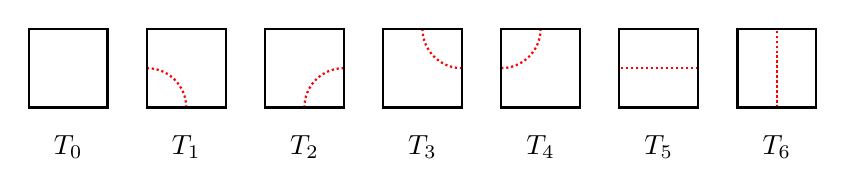
\begin{tikzpicture}
        \cell{0}{0}{1}{1}
        \( \lablnode{0.5}{-0.5}{$T_0$} \) 
        \cellA{1.5}{0}{2.5}{1}
        \( \lablnode{2}{-0.5}{$T_1$} \) 
        \cellB{3}{0}{4}{1}
        \( \lablnode{3.5}{-0.5}{$T_2$} \) 
        \cellC{4.5}{0}{5.5}{1}
        \( \lablnode{5}{-0.5}{$T_3$} \) 
        \cellD{6}{0}{7}{1}
        \( \lablnode{6.5}{-0.5}{$T_4$} \) 
        \cellE{7.5}{0}{8.5}{1}
        \( \lablnode{8}{-0.5}{$T_5$} \) 
        \cellF{9}{0}{10}{1}
        \( \lablnode{9.5}{-0.5}{$T_6$} \) 
        % \cellG{10.5}{0}{11.5}{1}
        % \( \lablnode{11}{-0.5}{$T_7$} \) 
        % \cellH{12}{0}{13}{1}
        % \( \lablnode{12.5}{-0.5}{$T_8$} \) 
        % \cellI{13.5}{0}{14.5}{1}
        % \( \lablnode{14}{-0.5}{$T_{9}$} \) 
        % \cellJ{15}{0}{16}{1}
        % \( \lablnode{15.5}{-0.5}{$T_{10}$} \) 
    \end{tikzpicture}
\end{center}
\caption{The tile set $\mathbb{T}$}
\label{fig:tile set}
\end{figure}

We denote the set of tiles $\mathbb{T}=\{T_0, \dots, T_{6}\}$. An $(m,n)$ \textit{mosaic} is an $m \times n$ matrix made up of elements from $\mathbb{T}$. Figure \ref{fig:example mosaic} shows an example $(5,7)$ mosaic. We denote the set of all $(m,n)$ mosaics as $\mathbb{M}^{(m,n)}$. As there are $7$ elements in $\mathbb{T}$, there are $7^{mn}$ mosaics in $\mathbb{M}^{(m,n)}$. 
% A \textit{mosaic system} is then a subset of $\mathbb{M}^{(m,n)}$ with some property. 

\begin{figure}[h!]
    \begin{center}
    \begin{subfigure}{0.4\textwidth}
        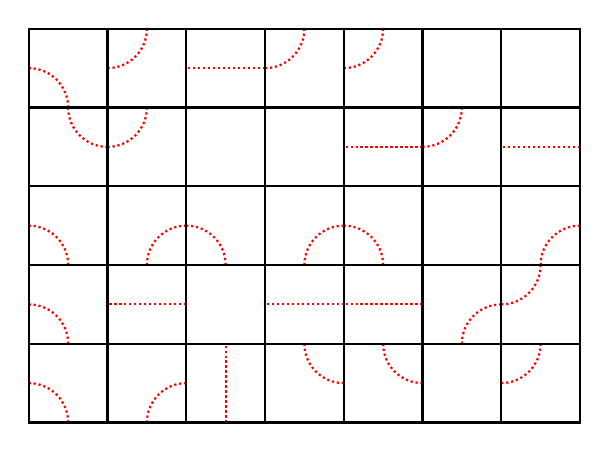
\begin{tikzpicture}
        % row1
        \cellA{0}{0}{1}{1}
        \cellB{1}{0}{2}{1}
        \cellF{2}{0}{3}{1}
        \cellC{3}{0}{4}{1}
        \cellC{4}{0}{5}{1}
        \cell{5}{0}{6}{1}
        \cellD{6}{0}{7}{1}
        % row2
        \cellA{0}{1}{1}{2}
        \cellE{1}{1}{2}{2}
        \cell{2}{1}{3}{2}
        \cellE{3}{1}{4}{2}
        \cellE{4}{1}{5}{2}
        \cellB{5}{1}{6}{2}
        \cellD{6}{1}{7}{2}
        % row3
        \cellA{0}{2}{1}{3}
        \cellB{1}{2}{2}{3}
        \cellA{2}{2}{3}{3}
        \cellB{3}{2}{4}{3}
        \cellA{4}{2}{5}{3}
        \cell{5}{2}{6}{3}
        \cellB{6}{2}{7}{3}
        % row4
        \cellC{0}{3}{1}{4}
        \cellD{1}{3}{2}{4}
        \cell{2}{3}{3}{4}
        \cell{3}{3}{4}{4}
        \cellE{4}{3}{5}{4}
        \cellD{5}{3}{6}{4}
        \cellE{6}{3}{7}{4}
        % row5
        \cellA{0}{4}{1}{5}
        \cellD{1}{4}{2}{5}
        \cellE{2}{4}{3}{5}
        \cellD{3}{4}{4}{5}
        \cellD{4}{4}{5}{5}
        \cell{5}{4}{6}{5}
        \cell{6}{4}{7}{5}
        \end{tikzpicture}
    \caption{A mosaic}
    \label{fig:example mosaic}
    \end{subfigure}
% \hfill
\hspace{0.05\textwidth}
\begin{subfigure}{0.4\textwidth}
    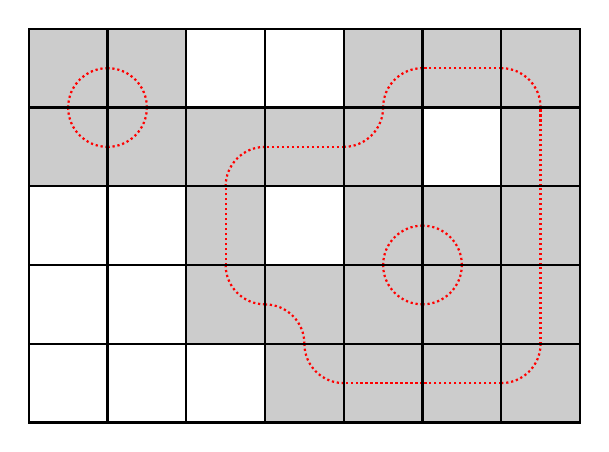
\begin{tikzpicture}
        % row1
        \cell{0}{0}{1}{1}
        \cell{1}{0}{2}{1}
        \cell{2}{0}{3}{1}
        \cellCf{3}{0}{4}{1}
        \cellEf{4}{0}{5}{1}
        \cellEf{5}{0}{6}{1}
        \cellDf{6}{0}{7}{1}
        % row2
        \cell{0}{1}{1}{2}
        \cell{1}{1}{2}{2}
        \cellCf{2}{1}{3}{2}
        \cellAf{3}{1}{4}{2}
        \cellCf{4}{1}{5}{2}
        \cellDf{5}{1}{6}{2}
        \cellFf{6}{1}{7}{2}
        % row3
        \cell{0}{2}{1}{3}
        \cell{1}{2}{2}{3}
        \cellFf{2}{2}{3}{3}
        \cell{3}{2}{4}{3}
        \cellBf{4}{2}{5}{3}
        \cellAf{5}{2}{6}{3}
        \cellFf{6}{2}{7}{3}
        % row4
        \cellCf{0}{3}{1}{4}
        \cellDf{1}{3}{2}{4}
        \cellBf{2}{3}{3}{4}
        \cellEf{3}{3}{4}{4}
        \cellDf{4}{3}{5}{4}
        \cell{5}{3}{6}{4}
        \cellFf{6}{3}{7}{4}
        % row5
        \cellBf{0}{4}{1}{5}
        \cellAf{1}{4}{2}{5}
        \cell{2}{4}{3}{5}
        \cell{3}{4}{4}{5}
        \cellBf{4}{4}{5}{5}
        \cellEf{5}{4}{6}{5}
        \cellAf{6}{4}{7}{5}
    \end{tikzpicture}
    \caption{A polygon mosaic}
    \label{fig:example polygon mosaic}
\end{subfigure}

\end{center}
\caption{Examples of mosaics of size $(5,7)$ made of tiles in $\mathbb{T}$}
\label{fig:example mosaics}
\end{figure}

The authors in \cite{Hong2018} are interested in mosaics with the property of being \textit{suitably connected}, which is defined as follows. Consider an edge shared between two tiles in Figure \ref{fig:example mosaic}. The edge has either $0$, $1$, or $2$ dotted lines drawn from its midpoint. Also note that the outer edges of the tiles on the boundary of the matrix are not shared by another tile. Therefore these edges only have $0$ or $1$ dotted lines drawn from their midpoint. A mosaic is suitably connected if all edges have $0$ or $2$ dotted lines drawn from their midpoint. The authors call these \textit{polygon mosaics} because, other than the mosaic consisting of all $T_0$ tiles, the dotted lines form \textit{polygons}.

\begin{definition}
    A \textit{polygon} $\mathcal{P}$ in a mosaic $\mathcal{M}$ is a non-empty subset of tiles in $\mathcal{M}$ such that if all cells in $\mathcal{P}^c$ are removed from $\mathcal{M}$, all remaining edges shared by $2$ tiles have $2$ dotted lines drawn from the midpoint, and all other edges have $0$ dotted lines drawn from their midpoint.\footnote{Polygons are more commonly refered to as ``self-avoiding polygons" in the literature to highlight their connection with self-avoiding walks.}
\end{definition}

\begin{exmp}
Figure \ref{fig:example polygon mosaic} shows a polygon $(5,7)$ mosaic that contains $3$ polygons, with the background of the tiles that make up the polygons highlighted in gray. Note that a mosaic can contain polygons that surround other polygons, such as in Figure \ref{fig:example polygon mosaic}. 

\begin{figure}[h!]
\begin{center}
    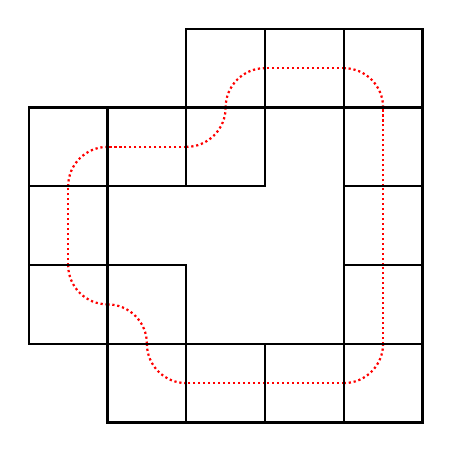
\begin{tikzpicture}
        % row1
        \cellC{3}{0}{4}{1}
        \cellE{4}{0}{5}{1}
        \cellE{5}{0}{6}{1}
        \cellD{6}{0}{7}{1}
        % row2
        \cellC{2}{1}{3}{2}
        \cellA{3}{1}{4}{2}
        \cellF{6}{1}{7}{2}
        % row3
        \cellF{2}{2}{3}{3}
        \cellF{6}{2}{7}{3}
        % row4
        \cellB{2}{3}{3}{4}
        \cellE{3}{3}{4}{4}
        \cellD{4}{3}{5}{4}
        \cellF{6}{3}{7}{4}
        % row5
        \cellB{4}{4}{5}{5}
        \cellE{5}{4}{6}{5}
        \cellA{6}{4}{7}{5}
    \end{tikzpicture}
\caption{The largest polygon in Figure \ref{fig:example polygon mosaic}}
\label{fig: example polygon}
\end{center}
\end{figure}
\end{exmp}

Using the notation conventions in \cite{Oh2014}, we denote the subset of $(m,n)$ mosaics that are polygon mosaics\footnote{The array of values of $\mathbb{P}^{(m,n)}$ is sequence A181245 on the OEIS \cite[OEIS]{oeis}.} as $\mathbb{P}^{(m,n)}$.

\begin{thm}[\cite{Hong2018}]
    \label{thm:Hong2018}
    The number of polygon $(m,n)$ mosaics $|\mathbb{P}^{(m,n)}|$ is bounded by
    $$2^{m+n-3}\left(\frac{17}{10}\right)^{(m-2)(n-2)} \leq |\mathbb{P}^{(m,n)}| \leq 2^{m+n-3}\left(\frac{31}{16}\right)^{(m-2)(n-2)}.$$
\end{thm}

This work follows \cite{Hong2018}, in that we do not consider the mosaic composed of all $T_0$ tiles a polygon mosaic, even though it is suitably connected. The authors \cite{Hong2018} point out Theorem \ref{thm:Hong2018} holds irrespective of this choice.

In related work, Lomonaco and Kauffman \cite{Lomonaco08} introduced mosaics constructed from a tile set of $11$ distinct tiles, of which $\mathbb{T}$ is a subset. The authors call mosaics constructed from this tile set that are suitably connected \textit{knot mosaics}. Oh et al. \cite{Oh2014} enumerated the number of knot mosaics.

\begin{thm}[\cite{Oh2014}]
    \label{thm:Oh2014}
    The number of knot mosaics of size $(m,n)$ for $m,n \geq 2$ is $2 \left\| (X_{m-2}+O_{m-2})^{n-2} \right\|$, where $X_0 = O_0 = \begin{bmatrix} 1 \\ \end{bmatrix}$ and $X_{m-2}$ and $O_{m-2}$ are $2^{m-2} \times 2^{m-2}$ matrices defined as

    $$ X_{k+1} = \begin{bmatrix}
        X_k & O_k \\
        O_k & X_k
    \end{bmatrix}
    \text{ and }
    O_{k+1} = \begin{bmatrix}
        O_k & X_k \\
        X_k & 4O_k
    \end{bmatrix}, $$
    
    for $k=0,1,\dots,m-3$. Here $\left\| N \right\|$ denotes the sum of elements of matrix $N$.
\end{thm}

Oh and colleagues refer to these matrices $X_k$ and $O_k$ as \textit{state matrices}. The authors utilize this state matrix recursion to bound the growth rate of knot mosaics \cite{Oh2016, Oh2019, Choi2024}, and Oh further adapts the method to solve problems in monomer and dimer tilings \cite{Oh2018Aztec, Oh2019tiling}. An unexamined direction in this research program is modifying the suitably connected property. This motivates us to introduce \textit{messy polygon mosaics} using the tiles set $\mathbb{T}$ from \cite{Hong2018}, and enumerate them with state matrices as in \cite{Oh2014}.

\section{Messy Polygon Mosaics}\label{section:messy mosaics}

\begin{definition}
    A \textit{messy polygon mosaic} is a mosaic that contains at least one polygon. 
\end{definition}

Figure \ref{fig:messy mosaic example} shows two examples of messy polygon $(5,7)$ mosaics that contain $3$ polygons. In both examples, we highlight the background of the tiles that make up each polygon in gray.

\begin{figure}[h!]
    \begin{center}

\begin{subfigure}{0.4\textwidth}
    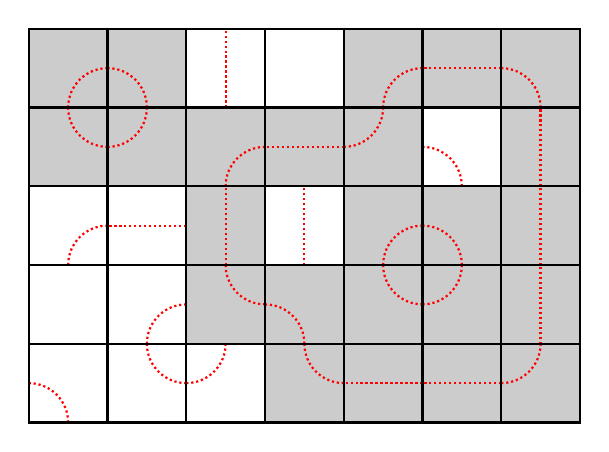
\begin{tikzpicture}
       % row1
        \cellA{0}{0}{1}{1}
        \cellC{1}{0}{2}{1}
        \cellD{2}{0}{3}{1}
        \cellCf{3}{0}{4}{1}
        \cellEf{4}{0}{5}{1}
        \cellEf{5}{0}{6}{1}
        \cellDf{6}{0}{7}{1}
        % row2
        \cell{0}{1}{1}{2}
        \cellB{1}{1}{2}{2}
        \cellCf{2}{1}{3}{2}
        \cellAf{3}{1}{4}{2}
        \cellCf{4}{1}{5}{2}
        \cellDf{5}{1}{6}{2}
        \cellFf{6}{1}{7}{2}
        % row3
        \cellB{0}{2}{1}{3}
        \cellE{1}{2}{2}{3}
        \cellFf{2}{2}{3}{3}
        \cellF{3}{2}{4}{3}
        \cellBf{4}{2}{5}{3}
        \cellAf{5}{2}{6}{3}
        \cellFf{6}{2}{7}{3}
        % row4
        \cellCf{0}{3}{1}{4}
        \cellDf{1}{3}{2}{4}
        \cellBf{2}{3}{3}{4}
        \cellEf{3}{3}{4}{4}
        \cellDf{4}{3}{5}{4}
        \cellA{5}{3}{6}{4}
        \cellFf{6}{3}{7}{4}
        % row5
        \cellBf{0}{4}{1}{5}
        \cellAf{1}{4}{2}{5}
        \cellF{2}{4}{3}{5}
        \cell{3}{4}{4}{5}
        \cellBf{4}{4}{5}{5}
        \cellEf{5}{4}{6}{5}
        \cellAf{6}{4}{7}{5}
    \end{tikzpicture}
\end{subfigure}
% \hfill
\hspace{0.05\textwidth}
\begin{subfigure}{0.4\textwidth}
        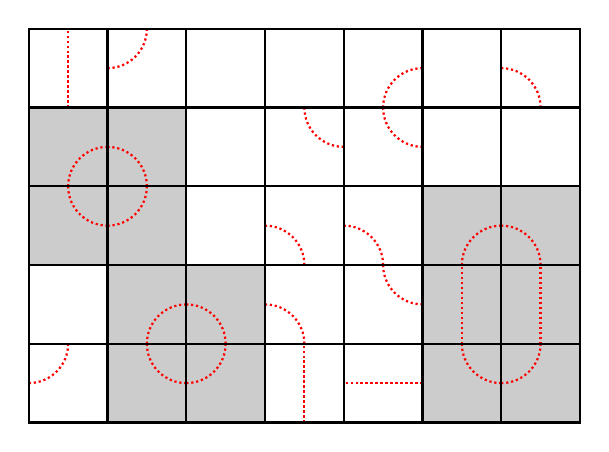
\begin{tikzpicture}
        % row1
        \cellD{0}{0}{1}{1}
        \cellCf{1}{0}{2}{1}
        \cellDf{2}{0}{3}{1}
        \cellF{3}{0}{4}{1}
        \cellE{4}{0}{5}{1}
        \cellCf{5}{0}{6}{1}
        \cellDf{6}{0}{7}{1}
        % row2
        \cell{0}{1}{1}{2}
        \cellBf{1}{1}{2}{2}
        \cellAf{2}{1}{3}{2}
        \cellA{3}{1}{4}{2}
        \cellC{4}{1}{5}{2}
        \cellFf{5}{1}{6}{2}
        \cellFf{6}{1}{7}{2}
        % row3
        \cellCf{0}{2}{1}{3}
        \cellDf{1}{2}{2}{3}
        \cell{2}{2}{3}{3}
        \cellA{3}{2}{4}{3}
        \cellA{4}{2}{5}{3}
        \cellBf{5}{2}{6}{3}
        \cellAf{6}{2}{7}{3}
        % row4
        \cellBf{0}{3}{1}{4}
        \cellAf{1}{3}{2}{4}
        \cell{2}{3}{3}{4}
        \cellC{3}{3}{4}{4}
        \cellC{4}{3}{5}{4}
        \cell{5}{3}{6}{4}
        \cell{6}{3}{7}{4}
        % row5
        \cellF{0}{4}{1}{5}
        \cellD{1}{4}{2}{5}
        \cell{2}{4}{3}{5}
        \cell{3}{4}{4}{5}
        \cellB{4}{4}{5}{5}
        \cell{5}{4}{6}{5}
        \cellA{6}{4}{7}{5}
    \end{tikzpicture}
\end{subfigure}

\end{center}
\caption{Messy polygon mosaics}
\label{fig:messy mosaic example}
\end{figure}

The main goal of this paper is to enumerate messy polygon mosaics, but it turns out to be simpler to enumerate the number of mosaics that \textit{do not} contain a polygon. Therefore, let $\mathbb{S}^{(m,n)}$ be the subset of mosaics that do not contain a polygon. Clearly the number of messy polygon mosaics is then $7^{mn} - |\mathbb{S}^{(m,n)}|$.

From the fact that the smallest polygon is made of $4$ tiles, shown in Figure \ref{fig:smallest polygon}, we can conclude that $|\mathbb{S}^{(n,1)}|=7^n$, and $|\mathbb{S}^{(2,2)}| = 7^4 - 1$. For $n,m \geq 2$, we first define the state matrices for messy polygon mosaics.

\begin{figure}[h!]
    \begin{center}
    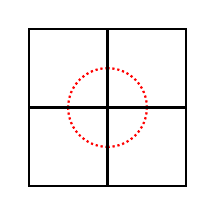
\begin{tikzpicture}
        % row1
        \cellC{0}{0}{1}{1}
        \cellD{1}{0}{2}{1}
        % row2
        \cellB{0}{1}{1}{2}
        \cellA{1}{1}{2}{2}
    \end{tikzpicture}
    \end{center}
    \caption{The smallest polygon}
    \label{fig:smallest polygon}
\end{figure}

\begin{definition}

Define $A^{(1,2)} = \begin{bmatrix}
7^2 & -1 \\
1 & 1
\end{bmatrix}$. We recursively define $A^{(1,k+1)} \in \mathbb{Z}^{2^{k} \times 2^{k}}$ given $A^{(1,k)}$. Begin by writing
$
A^{(1,k)} = \begin{bmatrix}
A_{[0,0]} & A_{[0,1]} \\
A_{[1,0]} & A_{[1,1]}
\end{bmatrix}
$, where the block matrices $A_{[i,j]}$ are square block matrices of size $2^{k-1} \times 2^{k-1}$. We then define

$$
A^{(1,k+1)} = \begin{bmatrix*}[r]
    7A_{[0,0]} & 7A_{[0,1]} & 7^{-1}A_{[0,0]} & A_{[0,1]} \\
    7A_{[1,0]} & 7A_{[1,1]} & 0A_{[1,0]} & A_{[1,1]} \\
    -7^{-1}A_{[0,0]} & 0A_{[0,1]} & 7^{-1}A_{[0,0]} & A_{[0,1]} \\
    A_{[1,0]} & A_{[1,1]} & -A_{[1,0]} & 7A_{[1,1]} \\
\end{bmatrix*}.
$$

\end{definition}

\begin{thm}
\label{thm: messy mosaics}
$|\mathbb{S}^{(m,n)}|$ is the $(0,0)$ entry of $(A^{(1,m)})^n$.
\end{thm}

\section{Preliminaries}

We begin by defining a mapping $f$ between $\mathbb{M}^{(m,n)}$ to a \textit{binary lattice} of size $(m,n)$. A binary lattice of size $(m,n)$ is a rectangular lattice of $m+1$ by $n+1$ vertices, in which the boundary vertices are labeled $0$, and the interior vertices are either $0$ or $1$. An example of a binary lattice of size $(5,7)$ is shown on the right of Figure \ref{fig:example of f mapping}. Also let $\mathbb{L}^{(m,n)}$ be the set of all binary lattices of size $(m,n)$, which gives $\left|\mathbb{L}^{(m,n)}\right| = 2^{(m-1)(n-1)}$. 

\begin{definition}

$f: \mathbb{M}^{(m,n)} \to \mathbb{L}^{(m,n)}$ takes a mosaic and labels each vertex with the following rule. If the vertex is surrounded by an even number of polygons (including $0$ polygons), label it $0$. If the vertex is surrounded by an odd number of polygons, label it $1$. Removing the red dotted lines from the tiles gives the binary lattice. 
    
\end{definition}

\begin{figure}
\begin{center}
    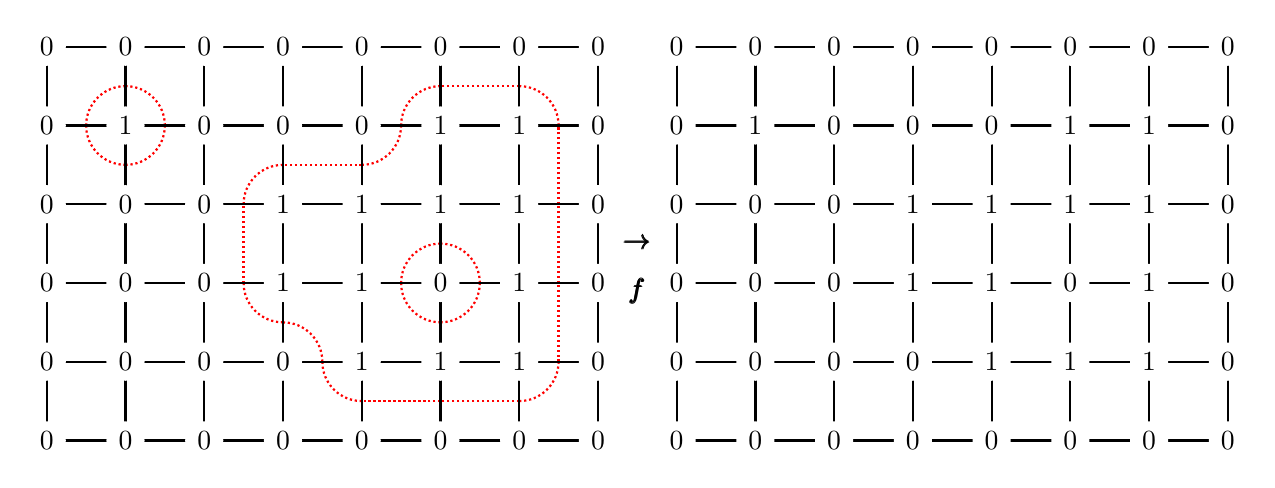
\begin{tikzpicture}
        % row1
        \cell{0}{0}{1}{1}
        \cell{1}{0}{2}{1}
        \cell{2}{0}{3}{1}
        \cellC{3}{0}{4}{1}
        \cellE{4}{0}{5}{1}
        \cellE{5}{0}{6}{1}
        \cellD{6}{0}{7}{1}
        % row2
        \cell{0}{1}{1}{2}
        \cell{1}{1}{2}{2}
        \cellC{2}{1}{3}{2}
        \cellA{3}{1}{4}{2}
        \cellC{4}{1}{5}{2}
        \cellD{5}{1}{6}{2}
        \cellF{6}{1}{7}{2}
        % row3
        \cell{0}{2}{1}{3}
        \cell{1}{2}{2}{3}
        \cellF{2}{2}{3}{3}
        \cell{3}{2}{4}{3}
        \cellB{4}{2}{5}{3}
        \cellA{5}{2}{6}{3}
        \cellF{6}{2}{7}{3}
        % row4
        \cellC{0}{3}{1}{4}
        \cellD{1}{3}{2}{4}
        \cellB{2}{3}{3}{4}
        \cellE{3}{3}{4}{4}
        \cellD{4}{3}{5}{4}
        \cell{5}{3}{6}{4}
        \cellF{6}{3}{7}{4}
        % row5
        \cellB{0}{4}{1}{5}
        \cellA{1}{4}{2}{5}
        \cell{2}{4}{3}{5}
        \cell{3}{4}{4}{5}
        \cellB{4}{4}{5}{5}
        \cellE{5}{4}{6}{5}
        \cellA{6}{4}{7}{5}
        % label for row1
        \( \lablvertex{0}{0}{$0$} \)
        \( \lablvertex{1}{0}{$0$} \)
        \( \lablvertex{2}{0}{$0$} \)
        \( \lablvertex{3}{0}{$0$} \)
        \( \lablvertex{4}{0}{$0$} \)
        \( \lablvertex{5}{0}{$0$} \)
        \( \lablvertex{6}{0}{$0$} \)
        \( \lablvertex{7}{0}{$0$} \)
        % label for row1
        \( \lablvertex{0}{1}{$0$} \)
        \( \lablvertex{1}{1}{$0$} \)
        \( \lablvertex{2}{1}{$0$} \)
        \( \lablvertex{3}{1}{$0$} \)
        \( \lablvertex{4}{1}{$1$} \)
        \( \lablvertex{5}{1}{$1$} \)
        \( \lablvertex{6}{1}{$1$} \)
        \( \lablvertex{7}{1}{$0$} \)
        % label for row1
        \( \lablvertex{0}{2}{$0$} \)
        \( \lablvertex{1}{2}{$0$} \)
        \( \lablvertex{2}{2}{$0$} \)
        \( \lablvertex{3}{2}{$1$} \)
        \( \lablvertex{4}{2}{$1$} \)
        \( \lablvertex{5}{2}{$0$} \)
        \( \lablvertex{6}{2}{$1$} \)
        \( \lablvertex{7}{2}{$0$} \)
        % label for row1
        \( \lablvertex{0}{3}{$0$} \)
        \( \lablvertex{1}{3}{$0$} \)
        \( \lablvertex{2}{3}{$0$} \)
        \( \lablvertex{3}{3}{$1$} \)
        \( \lablvertex{4}{3}{$1$} \)
        \( \lablvertex{5}{3}{$1$} \)
        \( \lablvertex{6}{3}{$1$} \)
        \( \lablvertex{7}{3}{$0$} \)
        % label for row1
        \( \lablvertex{0}{4}{$0$} \)
        \( \lablvertex{1}{4}{$1$} \)
        \( \lablvertex{2}{4}{$0$} \)
        \( \lablvertex{3}{4}{$0$} \)
        \( \lablvertex{4}{4}{$0$} \)
        \( \lablvertex{5}{4}{$1$} \)
        \( \lablvertex{6}{4}{$1$} \)
        \( \lablvertex{7}{4}{$0$} \)
        % label for row1
        \( \lablvertex{0}{5}{$0$} \)
        \( \lablvertex{1}{5}{$0$} \)
        \( \lablvertex{2}{5}{$0$} \)
        \( \lablvertex{3}{5}{$0$} \)
        \( \lablvertex{4}{5}{$0$} \)
        \( \lablvertex{5}{5}{$0$} \)
        \( \lablvertex{6}{5}{$0$} \)
        \( \lablvertex{7}{5}{$0$} \)
        % arrow
        \( \lablnode{7.5}{2.5}{$\pmb{\to}$} \)
        % 
        \( \lablnode{7.5}{1.9}{$\pmb{f}$} \)

        % row1
        \cell{8}{0}{9}{1}
        \cell{9}{0}{10}{1}
        \cell{10}{0}{11}{1}
        \cell{11}{0}{12}{1}
        \cell{12}{0}{13}{1}
        \cell{13}{0}{14}{1}
        \cell{14}{0}{15}{1}
        % row2
        \cell{8}{1}{9}{2}
        \cell{9}{1}{10}{2}
        \cell{10}{1}{11}{2}
        \cell{11}{1}{12}{2}
        \cell{12}{1}{13}{2}
        \cell{13}{1}{14}{2}
        \cell{14}{1}{15}{2}
        % row3
        \cell{8}{2}{9}{3}
        \cell{9}{2}{10}{3}
        \cell{10}{2}{11}{3}
        \cell{11}{2}{12}{3}
        \cell{12}{2}{13}{3}
        \cell{13}{2}{14}{3}
        \cell{14}{2}{15}{3}
        % row4
        \cell{8}{3}{9}{4}
        \cell{9}{3}{10}{4}
        \cell{10}{3}{11}{4}
        \cell{11}{3}{12}{4}
        \cell{12}{3}{13}{4}
        \cell{13}{3}{14}{4}
        \cell{14}{3}{15}{4}
        % row5
        \cell{8}{4}{9}{5}
        \cell{9}{4}{10}{5}
        \cell{10}{4}{11}{5}
        \cell{11}{4}{12}{5}
        \cell{12}{4}{13}{5}
        \cell{13}{4}{14}{5}
        \cell{14}{4}{15}{5}

        % label for row1
        \( \lablvertex{8}{0}{$0$} \)
        \( \lablvertex{9}{0}{$0$} \)
        \( \lablvertex{10}{0}{$0$} \)
        \( \lablvertex{11}{0}{$0$} \)
        \( \lablvertex{12}{0}{$0$} \)
        \( \lablvertex{13}{0}{$0$} \)
        \( \lablvertex{14}{0}{$0$} \)
        \( \lablvertex{15}{0}{$0$} \)
        % label for row1
        \( \lablvertex{8}{1}{$0$} \)
        \( \lablvertex{9}{1}{$0$} \)
        \( \lablvertex{10}{1}{$0$} \)
        \( \lablvertex{11}{1}{$0$} \)
        \( \lablvertex{12}{1}{$1$} \)
        \( \lablvertex{13}{1}{$1$} \)
        \( \lablvertex{14}{1}{$1$} \)
        \( \lablvertex{15}{1}{$0$} \)
        % label for row1
        \( \lablvertex{8}{2}{$0$} \)
        \( \lablvertex{9}{2}{$0$} \)
        \( \lablvertex{10}{2}{$0$} \)
        \( \lablvertex{11}{2}{$1$} \)
        \( \lablvertex{12}{2}{$1$} \)
        \( \lablvertex{13}{2}{$0$} \)
        \( \lablvertex{14}{2}{$1$} \)
        \( \lablvertex{15}{2}{$0$} \)
        % label for row1
        \( \lablvertex{8}{3}{$0$} \)
        \( \lablvertex{9}{3}{$0$} \)
        \( \lablvertex{10}{3}{$0$} \)
        \( \lablvertex{11}{3}{$1$} \)
        \( \lablvertex{12}{3}{$1$} \)
        \( \lablvertex{13}{3}{$1$} \)
        \( \lablvertex{14}{3}{$1$} \)
        \( \lablvertex{15}{3}{$0$} \)
        % label for row1
        \( \lablvertex{8}{4}{$0$} \)
        \( \lablvertex{9}{4}{$1$} \)
        \( \lablvertex{10}{4}{$0$} \)
        \( \lablvertex{11}{4}{$0$} \)
        \( \lablvertex{12}{4}{$0$} \)
        \( \lablvertex{13}{4}{$1$} \)
        \( \lablvertex{14}{4}{$1$} \)
        \( \lablvertex{15}{4}{$0$} \)
        % label for row1
        \( \lablvertex{8}{5}{$0$} \)
        \( \lablvertex{9}{5}{$0$} \)
        \( \lablvertex{10}{5}{$0$} \)
        \( \lablvertex{11}{5}{$0$} \)
        \( \lablvertex{12}{5}{$0$} \)
        \( \lablvertex{13}{5}{$0$} \)
        \( \lablvertex{14}{5}{$0$} \)
        \( \lablvertex{15}{5}{$0$} \)

    \end{tikzpicture}
\end{center}
\caption{$f$ applied to the left mosaic in Figure \ref{fig:messy mosaic example}, resulting in a binary lattice}
\label{fig:example of f mapping}
\end{figure}

Notice that by the definition of $f$, polygons draw out the boundary between edge-connected vertices with the same label, excluding the vertices that are edge-connected to the boundary $0$'s of the binary lattice. For example, in Figure \ref{fig:example of f mapping}, the three-polygons correspond with the three edge-connected regions of vertices that are not edge-connected to the boundary $0$'s.

To enumerate $|\mathbb{S}^{(m,n)}|$, it will be useful to consider how $f$ maps individual tiles in $\mathbb{T}$ to individual \textit{cells} in a binary lattice.

\begin{definition}
Let a \textit{cell} be the unit square and $4$ labeled vertices in a binary lattice that a given tile maps to.
\end{definition}

\begin{exmp}
\label{exmp: tile to cell}
Applying $f$ to the mosaic in Figure \ref{fig:example of f mapping}  results in the top-left tile $T_2$ mapping to the cell diagrammed below.

\begin{center}
    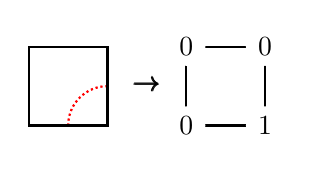
\begin{tikzpicture}
        \cellB{0}{0}{1}{1}
        
        \( \lablnode{1.5}{0.5}{$\pmb{\to}$} \)
        \cell{2}{0}{3}{1}
        
        \( \lablvertex{2}{0}{$0$} \)
        \( \lablvertex{2}{1}{$0$} \)
        \( \lablvertex{3}{0}{$1$} \)
        \( \lablvertex{3}{1}{$0$} \)
    \end{tikzpicture}
\end{center}
\end{exmp}

Let $C$ be the set of unique cells. For convenience, we give a pair of indexes to each of the $|C| = 2^4$ possible cells. The first index is the binary number formed by reading the bottom two vertices from left to right. The second index is the binary number formed by reading the top two vertices from left to right. The cell in Example \ref{exmp: tile to cell} has index $(01,00)$. Below is a diagram of all $2^4$ cells with their indexes listed below.

\begin{center}
    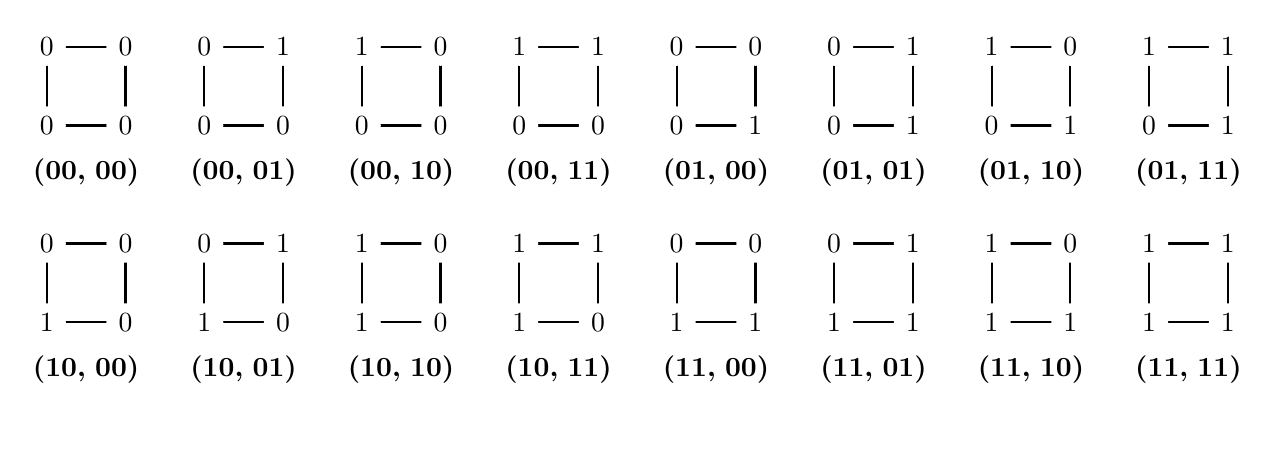
\begin{tikzpicture}
        % row1
        \cell{0}{-0.5}{1}{0.5}
        \cell{2}{-0.5}{3}{0.5}
        \cell{4}{-0.5}{5}{0.5}
        \cell{6}{-0.5}{7}{0.5}
        \cell{8}{-0.5}{9}{0.5}
        \cell{10}{-0.5}{11}{0.5}
        \cell{12}{-0.5}{13}{0.5}
        \cell{14}{-0.5}{15}{0.5}
        % row2
        \cell{0}{2}{1}{3}
        \cell{2}{2}{3}{3}
        \cell{4}{2}{5}{3}
        \cell{6}{2}{7}{3}
        \cell{8}{2}{9}{3}
        \cell{10}{2}{11}{3}
        \cell{12}{2}{13}{3}
        \cell{14}{2}{15}{3}

        % label for row 1
        \( \lablvertex{0}{-0.5}{$1$} \)
        \( \lablvertex{1}{-0.5}{$0$} \)
        \( \lablvertex{2}{-0.5}{$1$} \)
        \( \lablvertex{3}{-0.5}{$0$} \)
        \( \lablvertex{4}{-0.5}{$1$} \)
        \( \lablvertex{5}{-0.5}{$0$} \)
        \( \lablvertex{6}{-0.5}{$1$} \)
        \( \lablvertex{7}{-0.5}{$0$} \)
        \( \lablvertex{8}{-0.5}{$1$} \)
        \( \lablvertex{9}{-0.5}{$1$} \)
        \( \lablvertex{10}{-0.5}{$1$} \)
        \( \lablvertex{11}{-0.5}{$1$} \)
        \( \lablvertex{12}{-0.5}{$1$} \)
        \( \lablvertex{13}{-0.5}{$1$} \)
        \( \lablvertex{14}{-0.5}{$1$} \)
        \( \lablvertex{15}{-0.5}{$1$} \)
        
        % label for row 2
        \( \lablvertex{0}{0.5}{$0$} \)
        \( \lablvertex{1}{0.5}{$0$} \)
        \( \lablvertex{2}{0.5}{$0$} \)
        \( \lablvertex{3}{0.5}{$1$} \)
        \( \lablvertex{4}{0.5}{$1$} \)
        \( \lablvertex{5}{0.5}{$0$} \)
        \( \lablvertex{6}{0.5}{$1$} \)
        \( \lablvertex{7}{0.5}{$1$} \)
        \( \lablvertex{8}{0.5}{$0$} \)
        \( \lablvertex{9}{0.5}{$0$} \)
        \( \lablvertex{10}{0.5}{$0$} \)
        \( \lablvertex{11}{0.5}{$1$} \)
        \( \lablvertex{12}{0.5}{$1$} \)
        \( \lablvertex{13}{0.5}{$0$} \)
        \( \lablvertex{14}{0.5}{$1$} \)
        \( \lablvertex{15}{0.5}{$1$} \)

        % label for row 3
        \( \lablvertex{0}{2}{$0$} \)
        \( \lablvertex{1}{2}{$0$} \)
        \( \lablvertex{2}{2}{$0$} \)
        \( \lablvertex{3}{2}{$0$} \)
        \( \lablvertex{4}{2}{$0$} \)
        \( \lablvertex{5}{2}{$0$} \)
        \( \lablvertex{6}{2}{$0$} \)
        \( \lablvertex{7}{2}{$0$} \)
        \( \lablvertex{8}{2}{$0$} \)
        \( \lablvertex{9}{2}{$1$} \)
        \( \lablvertex{10}{2}{$0$} \)
        \( \lablvertex{11}{2}{$1$} \)
        \( \lablvertex{12}{2}{$0$} \)
        \( \lablvertex{13}{2}{$1$} \)
        \( \lablvertex{14}{2}{$0$} \)
        \( \lablvertex{15}{2}{$1$} \)
        
        % label for row 4
        \( \lablvertex{0}{3}{$0$} \)
        \( \lablvertex{1}{3}{$0$} \)
        \( \lablvertex{2}{3}{$0$} \)
        \( \lablvertex{3}{3}{$1$} \)
        \( \lablvertex{4}{3}{$1$} \)
        \( \lablvertex{5}{3}{$0$} \)
        \( \lablvertex{6}{3}{$1$} \)
        \( \lablvertex{7}{3}{$1$} \)
        \( \lablvertex{8}{3}{$0$} \)
        \( \lablvertex{9}{3}{$0$} \)
        \( \lablvertex{10}{3}{$0$} \)
        \( \lablvertex{11}{3}{$1$} \)
        \( \lablvertex{12}{3}{$1$} \)
        \( \lablvertex{13}{3}{$0$} \)
        \( \lablvertex{14}{3}{$1$} \)
        \( \lablvertex{15}{3}{$1$} \)

        % numbers row 1
        \( \lablnode{0.5}{1.4}{\textbf{(}$\mathbf{00}$\textbf{,} $\mathbf{00}$\textbf{)}} \)
        \( \lablnode{2.5}{1.4}{\textbf{(}$\mathbf{00}$\textbf{,} $\mathbf{01}$\textbf{)}} \)
        \( \lablnode{4.5}{1.4}{\textbf{(}$\mathbf{00}$\textbf{,} $\mathbf{10}$\textbf{)}} \)
        \( \lablnode{6.5}{1.4}{\textbf{(}$\mathbf{00}$\textbf{,} $\mathbf{11}$\textbf{)}} \)
        \( \lablnode{8.5}{1.4}{\textbf{(}$\mathbf{01}$\textbf{,} $\mathbf{00}$\textbf{)}} \)
        \( \lablnode{10.5}{1.4}{\textbf{(}$\mathbf{01}$\textbf{,} $\mathbf{01}$\textbf{)}} \)
        \( \lablnode{12.5}{1.4}{\textbf{(}$\mathbf{01}$\textbf{,} $\mathbf{10}$\textbf{)}} \)
        \( \lablnode{14.5}{1.4}{\textbf{(}$\mathbf{01}$\textbf{,} $\mathbf{11}$\textbf{)}} \)
        
        % numbers row 2
        \( \lablnode{0.5}{-1.1}{\textbf{(}$\mathbf{10}$\textbf{,} $\mathbf{00}$\textbf{)}} \)
        \( \lablnode{2.5}{-1.1}{\textbf{(}$\mathbf{10}$\textbf{,} $\mathbf{01}$\textbf{)}} \)
        \( \lablnode{4.5}{-1.1}{\textbf{(}$\mathbf{10}$\textbf{,} $\mathbf{10}$\textbf{)}} \)
        \( \lablnode{6.5}{-1.1}{\textbf{(}$\mathbf{10}$\textbf{,} $\mathbf{11}$\textbf{)}} \)
        \( \lablnode{8.5}{-1.1}{\textbf{(}$\mathbf{11}$\textbf{,} $\mathbf{00}$\textbf{)}} \)
        \( \lablnode{10.5}{-1.1}{\textbf{(}$\mathbf{11}$\textbf{,} $\mathbf{01}$\textbf{)}} \)
        \( \lablnode{12.5}{-1.1}{\textbf{(}$\mathbf{11}$\textbf{,} $\mathbf{10}$\textbf{)}} \)
        \( \lablnode{14.5}{-1.1}{\textbf{(}$\mathbf{11}$\textbf{,} $\mathbf{11}$\textbf{)}} \)
    \end{tikzpicture}
\end{center}

From the definition of $f$, mosaics that do not contain a polygon all map to the binary lattice of all $(00,00)$ cells.

\begin{definition}
    Let $\ell^*$ be the binary lattice made up of all $(00,00)$ cells.
    \label{def:all zeros}
\end{definition}

Therefore, we have

\begin{equation}
\label{eq: guiding eq}
|\mathbb{S}^{(m,n)}| = |f^{-1}(\{\ell^*\})|.
\end{equation}

Therefore, we need a way to compute $|f^{-1}(\{\ell\})|$ for a given binary lattice $\ell$. We begin by examining the number of tiles in $\mathbb{T}$ that can map to cell $(i,j)$, which we denote $u_{(i,j)}$. These values are simple to calculate, as each tile in $\mathbb{T}$ can only be part of a polygon in certain ways. For example, $u_{(01, 00)} = 1$, as cell $(01,00)$ can only be formed by a mosaic with $T_2$ in that location. We can see that $u_{(01,10)}=0$, as cell $(01,10)$ cannot be formed from any tiles in $\mathbb{T}$. Finally, we have $u_{(00,00)}=7$, as any tile can fail to contribute to forming a polygon. Table \ref{tbl:Preimage of binary cell lattice} summarizes the tiles in the preimage for each cell $(i,j)$. 

\begin{table}[h!]
    \begin{center}
        \begin{tabular}{ |c|l|c|c|l|c| } 
            \hline
            \textbf{Cell (}$\mathbf{i}$\textbf{,} $\mathbf{j}$\textbf{)} & \textbf{Preimage} & $\mathbf{u_{(i,j)}}$ & \textbf{Cell (}$\mathbf{i}$\textbf{,} $\mathbf{j}$\textbf{)} & \textbf{Preimage} & $\mathbf{u_{(i,j)}}$ \\ 
            \hline
            $(00, 00)$ & $\mathbb{T}$ & $7$ & $(11, 11)$ & $\mathbb{T}$ & $7$ \\
            \hline
            $(00, 01)$ & $\{T_3\}$ & $1$ & $(11, 10)$ & $\{T_3\}$ & $1$ \\
            \hline
            $(00, 10)$ & $\{T_4\}$ & $1$ & $(11, 01)$ & $\{T_4\}$ & $1$ \\
            \hline
            $(00, 11)$ & $\{T_5\}$ & $1$ & $(11, 00)$ & $\{T_5\}$ & $1$ \\
            \hline
            $(01, 00)$ & $\{T_2\}$ & $1$ & $(10, 11)$ & $\{T_2\}$ & $1$ \\
            \hline
            $(01, 01)$ & $\{T_6\}$ & $1$ & $(10, 10)$ & $\{T_6\}$ & $1$ \\
            \hline
            $(01, 10)$ & $\{\}$ & $0$ & $(10, 01)$ & $\{\}$ & $0$ \\
            \hline
            $(01, 11)$ & $\{T_1\}$ & $1$ & $(10, 00)$ & $\{T_1\}$ & $1$ \\
            \hline
        \end{tabular}
        \caption{Preimages of each unique cell under $f$}
        \label{tbl:Preimage of binary cell lattice}
    \end{center}
\end{table}

However, for some binary lattice $\ell$ the quantity 

\begin{equation}
    U(\ell) := \prod_{\text{Cell }(i,j) \in \ell} u_{(i,j)}
\end{equation}
is not necessarily equal to $\left|f^{-1}\left(\{\ell\}\right)\right|$, as $U(\ell)$ does not \textit{just} count the number of mosaics that map to $\ell$ under $f$. 

\begin{exmp}
    We have $U(\ell^*) = 7^{mn} = |\mathbb{M}^{(m,n)}|$, which clearly overcounts $|\mathbb{S}^{(m,n)}|$.
\label{eq: U doesnt work l star}
\end{exmp}

\begin{exmp}

Consider the following binary lattices and mosaics for $m=4,n=2$. 

\begin{center}
    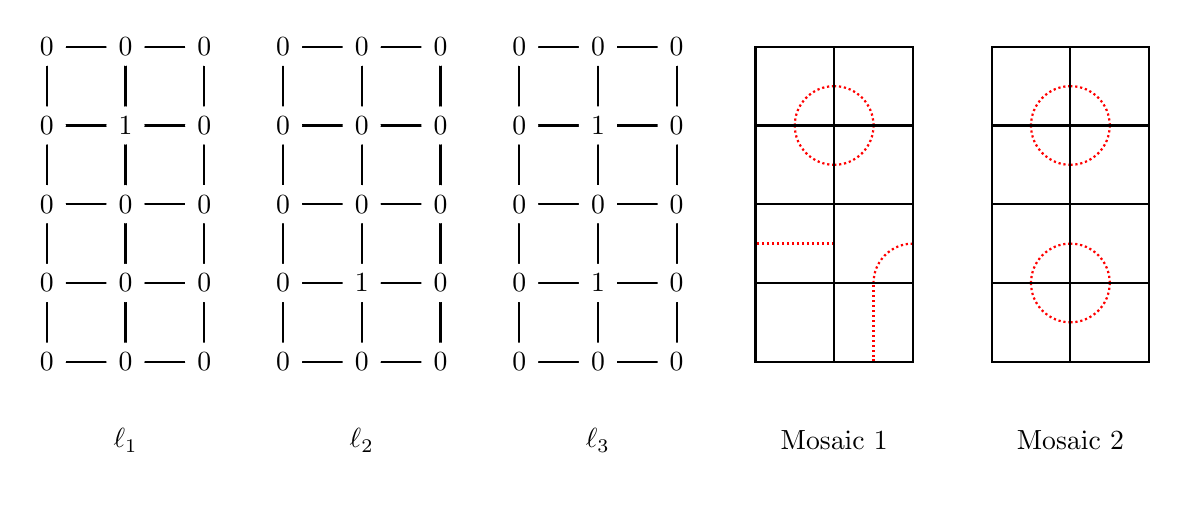
\begin{tikzpicture}

        % row1
        \cell{-3}{0}{-2}{1}
        \cell{-3}{1}{-2}{2}
        \cell{-3}{2}{-2}{3}
        \cell{-3}{3}{-2}{4}
        \cell{-2}{0}{-1}{1}
        \cell{-2}{1}{-1}{2}
        \cell{-2}{2}{-1}{3}
        \cell{-2}{3}{-1}{4}

        \( \lablnode{-2}{-1}{$\ell_{1}$} \)

        \( \lablvertex{-3}{0}{$0$} \)
        \( \lablvertex{-2}{0}{$0$} \)
        \( \lablvertex{-1}{0}{$0$} \)

        \( \lablvertex{-3}{1}{$0$} \)
        \( \lablvertex{-2}{1}{$0$} \)
        \( \lablvertex{-1}{1}{$0$} \)

        \( \lablvertex{-3}{2}{$0$} \)
        \( \lablvertex{-2}{2}{$0$} \)
        \( \lablvertex{-1}{2}{$0$} \)

        \( \lablvertex{-3}{3}{$0$} \)
        \( \lablvertex{-2}{3}{$1$} \)
        \( \lablvertex{-1}{3}{$0$} \)

        \( \lablvertex{-3}{4}{$0$} \)
        \( \lablvertex{-2}{4}{$0$} \)
        \( \lablvertex{-1}{4}{$0$} \)

        % row1
        \cell{0}{0}{1}{1}
        \cell{0}{1}{1}{2}
        \cell{0}{2}{1}{3}
        \cell{0}{3}{1}{4}
        \cell{1}{0}{2}{1}
        \cell{1}{1}{2}{2}
        \cell{1}{2}{2}{3}
        \cell{1}{3}{2}{4}

        \( \lablnode{1}{-1}{$\ell_{2}$} \)
        
        \( \lablvertex{0}{0}{$0$} \)
        \( \lablvertex{1}{0}{$0$} \)
        \( \lablvertex{2}{0}{$0$} \)

        \( \lablvertex{0}{1}{$0$} \)
        \( \lablvertex{1}{1}{$1$} \)
        \( \lablvertex{2}{1}{$0$} \)

        \( \lablvertex{0}{2}{$0$} \)
        \( \lablvertex{1}{2}{$0$} \)
        \( \lablvertex{2}{2}{$0$} \)

        \( \lablvertex{0}{3}{$0$} \)
        \( \lablvertex{1}{3}{$0$} \)
        \( \lablvertex{2}{3}{$0$} \)

        \( \lablvertex{0}{4}{$0$} \)
        \( \lablvertex{1}{4}{$0$} \)
        \( \lablvertex{2}{4}{$0$} \)

        % row1
        \cell{3}{0}{4}{1}
        \cell{3}{1}{4}{2}
        \cell{3}{2}{4}{3}
        \cell{3}{3}{4}{4}
        \cell{4}{0}{5}{1}
        \cell{4}{1}{5}{2}
        \cell{4}{2}{5}{3}
        \cell{4}{3}{5}{4}

        \( \lablnode{4}{-1}{$\ell_{3}$} \)

        \( \lablvertex{3}{0}{$0$} \)
        \( \lablvertex{4}{0}{$0$} \)
        \( \lablvertex{5}{0}{$0$} \)

        \( \lablvertex{3}{1}{$0$} \)
        \( \lablvertex{4}{1}{$1$} \)
        \( \lablvertex{5}{1}{$0$} \)

        \( \lablvertex{3}{2}{$0$} \)
        \( \lablvertex{4}{2}{$0$} \)
        \( \lablvertex{5}{2}{$0$} \)

        \( \lablvertex{3}{3}{$0$} \)
        \( \lablvertex{4}{3}{$1$} \)
        \( \lablvertex{5}{3}{$0$} \)

        \( \lablvertex{3}{4}{$0$} \)
        \( \lablvertex{4}{4}{$0$} \)
        \( \lablvertex{5}{4}{$0$} \)

        \cell{6}{0}{7}{1}
        \cellF{7}{0}{8}{1}

        \cellE{6}{1}{7}{2}
        \cellB{7}{1}{8}{2}

        \cellC{6}{2}{7}{3}
        \cellD{7}{2}{8}{3}    

        \cellB{6}{3}{7}{4}
        \cellA{7}{3}{8}{4}    

        \( \lablnode{7}{-1}{Mosaic $1$} \)

        \cellC{9}{0}{10}{1}
        \cellD{10}{0}{11}{1}

        \cellB{9}{1}{10}{2}
        \cellA{10}{1}{11}{2}

        \cellC{9}{2}{10}{3}
        \cellD{10}{2}{11}{3}    

        \cellB{9}{3}{10}{4}
        \cellA{10}{3}{11}{4}    

        \( \lablnode{10}{-1}{Mosaic $2$} \)

    \end{tikzpicture}
\end{center}

We have $U(\ell_1) = 7^4, U(\ell_2) = 7^4,$ and $U(\ell_3) = 1$. $U(\ell_{1})$ uniquely counts Mosaic $1$, but both $U(\ell_{1})$ and $U(\ell_{2})$ count Mosaic $2$, for which $f(\text{Mosaic } 2) = \ell_3$. This is because each cell in the bottom two rows of $\ell_1$ could have come from $7$ possible cells, though $1$ of the $7^4$ permutations contains a new polygon. 

\label{exmp:U doesnt work}
\end{exmp}

Examples \ref{eq: U doesnt work l star} and \ref{exmp:U doesnt work} show we cannot compute $|f^{-1}(\{\ell\})|$ for a given binary lattice $\ell$ just by examining the cells of $\ell$. Therefore $U$ counts the number of mosaics that map to some set of binary lattices under $f$. This set is defined in Definition \ref{def: set u}.

\begin{definition}
A polygon is \textit{specified} by a binary lattice $\ell$ if all mosaics in $f^{-1}(\{\ell\})$ contain the polygon.
\end{definition}

\begin{definition}
Let $P: \mathbb{L}^{(m,n)} \to \mathbb{N}$ be the number of polygons specified in a binary lattice $\ell$.
\end{definition}

\begin{exmp}
From Example \ref{exmp:U doesnt work}, $\ell_1$ specifies the polygon in the top $2$ rows of Mosaic $1$ and Mosaic $2$, but not the polygon in the bottom $2$ rows of Mosaic $2$. $\ell_3$ specifies both polygons in Mosaic $2$. Therefore $P(\ell_1) = P(\ell_2) = 1$, and $P(\ell_3) = 2$.
\label{exmp:specifying example}
\end{exmp}

\begin{exmp}
The binary lattice $\ell^*$ specifies $0$ polygons, and so $P(\ell^*)=0$.
\end{exmp}

Notice that cells that specify a polygon must have $u_{(i,j)}=1$. 

\begin{definition}
For binary lattices $\ell, \ell'$, we say $\ell' \leq \ell$ if one can construct $\ell'$ by flipping the parity of some number of vertices (possibly $0$ vertices) in $\ell$, such that all polygons specified by $\ell$ are unchanged and no cells with index $(01,10)$ or $(10,01)$ are created.
\end{definition}

\begin{definition}
For a binary lattice $\ell$, let $\mathbb{U}(\ell) = \{\ell' | \ell' \leq \ell\}$.
\label{def: set u}
\end{definition}

\begin{exmp}
From Example \ref{exmp:U doesnt work}, $\ell_3 \leq \ell_1$ as one can construct $\ell_3$ from $\ell_1$ by flipping the vertex at $(3,1)$ from $0$ to $1$. As $\ell_1$ specifies the polygon in the top two rows of Mosaic $2$, and this vertex flip does not change the top polygon, $\ell_3 \leq \ell_1$. We also have $\ell_1 \leq \ell_1$ simply by selecting no vertices to flip. As diagrammed below, constructing $\ell_4$ from $\ell_1$ by flipping the vertex at $(2,1)$ does change a polygon specified by $\ell_1$, and so $\ell_4 \nleq \ell_1$.

% \begin{figure}[h!]
\begin{center}
    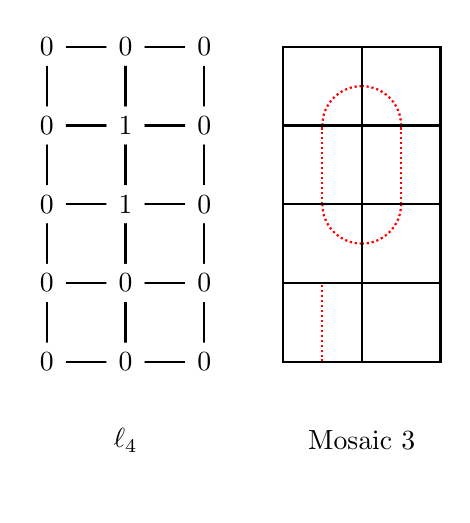
\begin{tikzpicture}
        % row1
        \cell{0}{0}{1}{1}
        \cell{0}{1}{1}{2}
        \cell{0}{2}{1}{3}
        \cell{0}{3}{1}{4}
        \cell{1}{0}{2}{1}
        \cell{1}{1}{2}{2}
        \cell{1}{2}{2}{3}
        \cell{1}{3}{2}{4}

        \( \lablnode{1}{-1}{$\ell_{4}$} \)

        \( \lablvertex{0}{0}{$0$} \)
        \( \lablvertex{1}{0}{$0$} \)
        \( \lablvertex{2}{0}{$0$} \)

        \( \lablvertex{0}{1}{$0$} \)
        \( \lablvertex{1}{1}{$0$} \)
        \( \lablvertex{2}{1}{$0$} \)

        \( \lablvertex{0}{2}{$0$} \)
        \( \lablvertex{1}{2}{$1$} \)
        \( \lablvertex{2}{2}{$0$} \)

        \( \lablvertex{0}{3}{$0$} \)
        \( \lablvertex{1}{3}{$1$} \)
        \( \lablvertex{2}{3}{$0$} \)

        \( \lablvertex{0}{4}{$0$} \)
        \( \lablvertex{1}{4}{$0$} \)
        \( \lablvertex{2}{4}{$0$} \)

        \cellF{3}{0}{4}{1}
        \cell{4}{0}{5}{1}

        \cellC{3}{1}{4}{2}
        \cellD{4}{1}{5}{2}

        \cellF{3}{2}{4}{3}
        \cellF{4}{2}{5}{3}    

        \cellB{3}{3}{4}{4}
        \cellA{4}{3}{5}{4}    

        \( \lablnode{4}{-1}{Mosaic $3$} \)

    \end{tikzpicture}
\end{center}
% \label{fig: ell 4}
% \caption{}
% \end{figure}

Therefore $\mathbb{U}(\ell_1) = \{\ell_1, \ell_3\}$. Additionally, $\mathbb{U}(\ell_2) = \{\ell_2, \ell_3\}$, and $\mathbb{U}(\ell_3) = \{\ell_3\}$.

\label{exmp:four two mosaics}
\end{exmp}

\begin{exmp}
Every binary lattice $\ell$ has $\ell \leq \ell^*$, as $\ell^*$ specifies no polygons. Therefore for a given $(m,n)$, we have $\mathbb{U}(\ell^*) = \mathbb{L}^{(m,n)}$.
\end{exmp}

\begin{prop}
$\mathbb{U}(\ell)$ is the set such that
\begin{equation}
U(\ell) = \sum_{\ell' \in \mathbb{U}(\ell)}|f^{-1}(\{\ell'\})|.
\label{eq:U identity}
\end{equation}
\label{prop:U counts mathbb U}
\end{prop}

\begin{proof}
For a binary lattice $\ell' \in \mathbb{U}(\ell)$, $\ell'$ specifies new polygons without changing any of the polygons specified in $\ell$. Denote the set of locations of the cells that specify the new polygons in $\ell'$ as $S$. Clearly these cells all have $u_{(i,j)}=1$. The cells in $\ell$ at $S$ must therefore be either cell $(00,00)$ or cell $(11,11)$, as otherwise the vertex flips would change atleast one polygon specified in $\ell$. As $u_{(00,00)} = u_{(11,11)} = |\mathbb{T}|$, $U(\ell)$ counts each possible tile configuration at $S$. Therefore, one of these contains the tiles that create the new polygons specified by $\ell'$, and so $\ell'$ is also counted by $U$.
\end{proof}

Surprisingly, we can recover $|\mathbb{M}^{(m,n)}| = |f^{-1}(\{\ell^*\})|$ by first considering how much each preimage of $\ell \in \mathbb{L}^{(m,n)}$ is over counted in 

\begin{equation}
    \sum_{\ell \in \mathbb{L}^{(m,n)}}U(\ell)
\end{equation}

in Proposition \ref{prop: over counting term}, then manipulating the sum in Proposition \ref{prop: recover total}.

\begin{prop}
    By regrouping terms we have

    \begin{equation}
        \sum_{\ell \in \mathbb{L}^{(m,n)}} U(\ell) = \sum_{\ell \in \mathbb{L}^{(m,n)}}\sum_{\ell' \in \mathbb{U}(\ell)}|f^{-1}(\{\ell'\})| = \sum_{\ell \in \mathbb{L}^{(m,n)}} \left(\sum_{p=0}^{P(\ell)}\binom{P(\ell)}{p}\right)|f^{-1}(\{\ell\})|.
        \label{eq:double counting terms}
    \end{equation}
\label{prop: over counting term}
\end{prop}

\begin{proof}
The first equality follows directly from Proposition \ref{prop:U counts mathbb U}. For the second equality, for a given binary lattice $\ell$ the coefficient of $|f^{-1}(\{\ell\})|$ is the number of elements in $\{\ell' | \ell \leq \ell'\}$. Therefore, a binary lattice is in $\{\ell' | \ell \leq \ell'\}$ if the binary lattice only specifies $0 \leq p \leq P(\ell)$ of the $P(\ell)$ polygons specified by $\ell$. As there are $\binom{P(\ell)}{p}$ ways to specify $p$ polygons from a choice of $P(\ell)$ polygons, this gives the second equality for all $P(\ell)>0$.

If $\ell'$ has $P(\ell') = 0$, then $\ell' = \ell^*$. As $\{\ell' | \ell^* \leq \ell'\} = \{\ell^*\}$, the term $|f^{-1}(\ell')|$ is only counted once. As $1=\binom{0}{0}$, this completes the proof.
\end{proof}

\begin{prop}
    The number of $(m,n)$ mosaics that do not contain a polygon $|\mathbb{S}^{(m,n)}|$ has

    \begin{equation}
    |\mathbb{S}^{(m,n)}| = \sum_{\ell \in \mathbb{L}^{(m,n)}} (-1)^{P(\ell)} U(\ell).
    \label{eq:ugly inc excl}
    \end{equation}
\label{prop: recover total}
\end{prop}

\begin{proof}
    By the binomial theorem, for $P(\ell) > 0$ we have
    
    $$0 = (1-1)^{P(\ell)} = \sum_{p=0}^{P(\ell)}(-1)^{P(\ell)}\binom{P(\ell)}{p}.$$
    
    If we group terms as in the second equality of Equation \ref{eq:double counting terms}, we get that all terms where $P(\ell)>0$ are $0$. As the only binary lattice with $P(\ell) = 0$ is $\ell^*$, we have
    
    $$\sum_{\ell \in \mathbb{L}^{(m,n)}} (-1)^{P(\ell)} U(\ell) = \binom{0}{0}|f^{-1}(\ell^*)| = |\mathbb{S}^{(m,n)}|.$$
\end{proof}

\section{A Cell-Level Identity}

Though Equation \ref{eq:ugly inc excl} does compute $|\mathbb{S}^{(m,n)}|$, computing the number of polygons specified in a binary lattice $P(\ell)$ requires examining the entire structure of $\ell$. It will be more efficient to recover the $(-1)^{P(\ell)}$ term at the level of individual cells. More concretely, we seek a function $V$ of the form

$$V(\ell) := \prod_{\text{Cell } (i,j) \in \ell} v_{(i,j)},$$

such that for all $\ell$

\begin{equation}
    (-1)^{P(\ell)}U(\ell) = V(\ell).
\label{eq:technically correct}
\end{equation}

The idea is to add a coefficient $p_{(i,j)} \in \{-1,1\}$ to each value of $u_{(i,j)}$ in such a way as to recover the $(-1)^{P(\ell)}$ term. With this in mind we define $v_{(i,j)} := p_{(i,j)}u_{(i,j)}$.

\begin{condition}
A subset of cells $\mathcal{S}$ in a binary lattice $\ell$ meets this condition if

\begin{equation}
    \prod_{\text{Cell } (i,j) \in \mathcal{S}} p_{(i,j)} = -1,
    \label{eq:neg prod polygon condition}
\end{equation}
with $p_{(i,j)} \in \{-1,1\}$.
\label{cond:neg prod condition}
\end{condition}

Cells in a binary lattice either do or do not specify a polygon. To recover the $(-1)^{P(\ell)}$ term, the following must be true. Cells that cannot specify a polygon must all have $p_{(i,j)}=1$. Moreover, if a set of cells specifies any one polygon, it must meet Condition \ref{cond:neg prod condition}.

\begin{prop}
There exists values $p_{(i,j)}$ for which the cells that do not specify a polygon have $p_{(i,j)}=1$, and Condition \ref{cond:neg prod condition} holds for any set of cells that specify a polygon.
\label{prop:neg prod prop}
\end{prop}

\begin{proof}

We can immediately see $p_{(00,00)} = p_{(11,11)} = p_{(01,10)} = p_{(10,01)} = 1$, as cells $(00,00)$, $(11,11)$, $(01,10)$, and $(10,01)$ can never be in the subset of cells that specify a polygon, and so must be positive.

For the remaining values of $p_{(i,j)}$, we first examine the cells that map to the smallest polygon, shown in Figure \ref{fig:smallest polygon}. 

\begin{figure}[h!]
\begin{center}
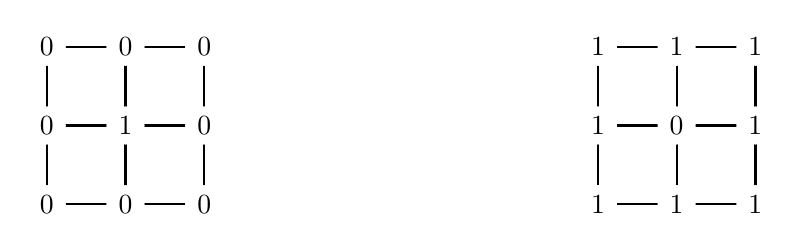
\begin{tikzpicture}
    % row1
    \cell{0}{0}{1}{1}
    \cell{1}{0}{2}{1}
    % row2
    \cell{0}{1}{1}{2}
    \cell{1}{1}{2}{2}
    % label for row1
    \( \lablvertex{0}{0}{$0$} \)
    \( \lablvertex{1}{0}{$0$} \)
    \( \lablvertex{2}{0}{$0$} \)
    % label for row2
    \( \lablvertex{0}{1}{$0$} \)
    \( \lablvertex{1}{1}{$1$} \)
    \( \lablvertex{2}{1}{$0$} \)
    % label for row3
    \( \lablvertex{0}{2}{$0$} \)
    \( \lablvertex{1}{2}{$0$} \)
    \( \lablvertex{2}{2}{$0$} \)

    % \( \lablnode{1}{-0.5}{$p_{(00,01)} p_{(00,10)} p_{(01,00)} p_{(10,00)} = -1$} \)

    % row1
    \cell{7}{0}{8}{1}
    \cell{8}{0}{9}{1}
    % row2
    \cell{7}{1}{8}{2}
    \cell{8}{1}{9}{2}
    % label for row1
    \( \lablvertex{7}{0}{$1$} \)
    \( \lablvertex{8}{0}{$1$} \)
    \( \lablvertex{9}{0}{$1$} \)
    % label for row2
    \( \lablvertex{7}{1}{$1$} \)
    \( \lablvertex{8}{1}{$0$} \)
    \( \lablvertex{9}{1}{$1$} \)
    % label for row3
    \( \lablvertex{7}{2}{$1$} \)
    \( \lablvertex{8}{2}{$1$} \)
    \( \lablvertex{9}{2}{$1$} \)
    
    % \( \lablnode{8}{-0.5}{$p_{(11,10)} p_{(11,01)} p_{(10,11)} p_{(01,11)} = -1$} \)
\end{tikzpicture}
\end{center}
\caption{Portions of binary lattices associated with the smallest polygon}
\label{fig:constraints i and ii}
\end{figure}

For the portions of binary lattices in Figure \ref{fig:constraints i and ii}, Condition \ref{cond:neg prod condition} amounts to the following two equations

\begin{equation}
  \begin{aligned}
  p_{(00,01)} p_{(00,10)} p_{(01,00)} p_{(10,00)} & = -1  \\
  p_{(11,10)} p_{(11,01)} p_{(10,11)} p_{(01,11)} & = -1.
  \end{aligned}
  \label{eq:constraints i and ii}
\end{equation}

We refer to the equations above as \textit{constraints}, as they constrain the possible assignments of $p_{(i,j)}$. %Let the constraints in Equation \ref{eq:constraints i and ii} be numbered $1$ and $2$.

To define the remaining constraints, consider the unbounded square lattice with all vertices labeled $0$, except for the origin labeled $1$. We refer to this as the \textit{starting position}.

From the definition of $f$ we know that polygons are the boundary of edge-connected vertices of the same label. Clearly one can construct arbitrary sets of edge-connected $0$'s and $1$'s from the starting position by flipping the parity of a vertex one-by-one.

This \textit{bit flip} operation, depicted in Figure \ref{fig:bit flip}, corresponds with changing the identity of the four cells that share that vertex. As each cell has its associated $p_{(i,j)}$ value, it must be the case that the bit flip preserves Condition \ref{cond:neg prod condition} for the cells involved. Additionally, as the surrounding $8$ vertices are unchanged udner this operation, we must define $2^8$ constraints.

In each of the constraints, the parity of the number of edge-connected regions of $1$s must either change or stay the same after the bit flip. If the parity remains unchanged, the bit flip is of \textit{Type 1}, and if the parity changes the bit flip is of \textit{Type 2}.

\begin{figure}[h!]
    \begin{center}

\begin{subfigure}{0.4\textwidth}
    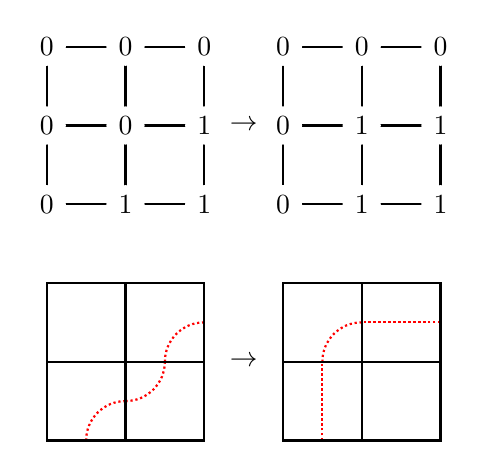
\begin{tikzpicture}
        % row1
        \cell{0}{0}{1}{1}
        \cell{1}{0}{2}{1}
        % row2
        \cell{0}{1}{1}{2}
        \cell{1}{1}{2}{2}
        % label for row1
        \( \lablvertex{0}{0}{$0$} \)
        \( \lablvertex{1}{0}{$1$} \)
        \( \lablvertex{2}{0}{$1$} \)
        % label for row2
        \( \lablvertex{0}{1}{$0$} \)
        \( \lablvertex{1}{1}{$0$} \)
        \( \lablvertex{2}{1}{$1$} \)
        % label for row3
        \( \lablvertex{0}{2}{$0$} \)
        \( \lablvertex{1}{2}{$0$} \)
        \( \lablvertex{2}{2}{$0$} \)
        % row1
        \cell{3}{0}{4}{1}
        \cell{4}{0}{5}{1}
        % row2
        \cell{3}{1}{4}{2}
        \cell{4}{1}{5}{2}
        % label for row1
        \( \lablvertex{3}{0}{$0$} \)
        \( \lablvertex{4}{0}{$1$} \)
        \( \lablvertex{5}{0}{$1$} \)
        % label for row2
        \( \lablvertex{3}{1}{$0$} \)
        \( \lablvertex{4}{1}{$1$} \)
        \( \lablvertex{5}{1}{$1$} \)
        % label for row3
        \( \lablvertex{3}{2}{$0$} \)
        \( \lablvertex{4}{2}{$0$} \)
        \( \lablvertex{5}{2}{$0$} \)

        \( \lablnode{2.5}{1}{$\rightarrow$} \)
        
        \cellB{0}{-3}{1}{-2}
        \cellD{1}{-3}{2}{-2}
        \cell{0}{-2}{1}{-1}
        \cellB{1}{-2}{2}{-1}
        
        \( \lablnode{2.5}{-2}{$\rightarrow$} \)

        \cellF{3}{-3}{4}{-2}
        \cell{4}{-3}{5}{-2}
        \cellB{3}{-2}{4}{-1}
        \cellE{4}{-2}{5}{-1}

    \end{tikzpicture}
    \caption{Type 1 bit flip and associated tiles}
    \label{fig:type 1 bit flip}
\end{subfigure}
% \hfill
\hspace{0.05\textwidth}
\begin{subfigure}{0.4\textwidth}
    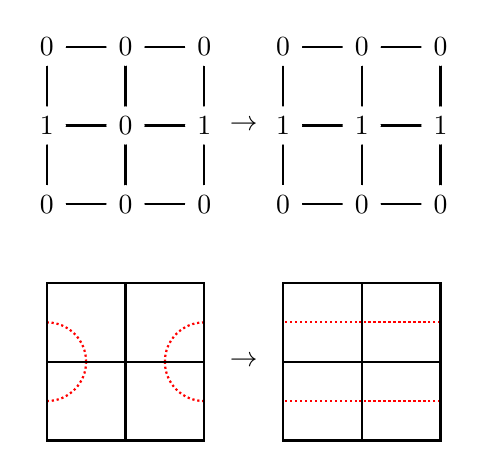
\begin{tikzpicture}
        % row1
        \cell{0}{0}{1}{1}
        \cell{1}{0}{2}{1}
        % row2
        \cell{0}{1}{1}{2}
        \cell{1}{1}{2}{2}
        % label for row1
        \( \lablvertex{0}{0}{$0$} \)
        \( \lablvertex{1}{0}{$0$} \)
        \( \lablvertex{2}{0}{$0$} \)
        % label for row2
        \( \lablvertex{0}{1}{$1$} \)
        \( \lablvertex{1}{1}{$0$} \)
        \( \lablvertex{2}{1}{$1$} \)
        % label for row3
        \( \lablvertex{0}{2}{$0$} \)
        \( \lablvertex{1}{2}{$0$} \)
        \( \lablvertex{2}{2}{$0$} \)
        
        % row1
        \cell{3}{0}{4}{1}
        \cell{4}{0}{5}{1}
        % row2
        \cell{3}{1}{4}{2}
        \cell{4}{1}{5}{2}
        % label for row1
        \( \lablvertex{3}{0}{$0$} \)
        \( \lablvertex{4}{0}{$0$} \)
        \( \lablvertex{5}{0}{$0$} \)
        % label for row2
        \( \lablvertex{3}{1}{$1$} \)
        \( \lablvertex{4}{1}{$1$} \)
        \( \lablvertex{5}{1}{$1$} \)
        % label for row3
        \( \lablvertex{3}{2}{$0$} \)
        \( \lablvertex{4}{2}{$0$} \)
        \( \lablvertex{5}{2}{$0$} \)

        \( \lablnode{2.5}{1}{$\rightarrow$} \)

        \cellD{0}{-3}{1}{-2}
        \cellC{1}{-3}{2}{-2}
        \cellA{0}{-2}{1}{-1}
        \cellB{1}{-2}{2}{-1}
        
        \( \lablnode{2.5}{-2}{$\rightarrow$} \)

        \cellE{3}{-3}{4}{-2}
        \cellE{4}{-3}{5}{-2}
        \cellE{3}{-2}{4}{-1}
        \cellE{4}{-2}{5}{-1}

    \end{tikzpicture}
    \caption{Type 2 bit flip and associated tiles}
    \label{fig:type 2 bit flip}
\end{subfigure}

\end{center}
\caption{Bit flips for binary lattices}
\label{fig:bit flip}
\end{figure}

For a bit flip of \textit{Type 1}, to adhere to Condition \ref{cond:neg prod condition}, the associated constraint is that the sign of the product of the related cells must stay the same after the flip. For example, Figure \ref{fig:type 1 bit flip} represents the constraint

\begin{equation}
    p_{(01,00)}p_{(11,01)}p_{(00,00)}p_{(01,00)} = p_{(01,01)}p_{(11,11)}p_{(01,00)}p_{(11,00)}.
\end{equation}

For a bit flip of \textit{Type 2}, to adhere to Condition \ref{cond:neg prod condition}, the associated constraint is that the sign of the product of the related cells must change after the flip. For example, Figure \ref{fig:type 2 bit flip} represents the constraint

\begin{equation}
    p_{(00,10)}p_{(00,01)}p_{(10,00)}p_{(01,00)} = -p_{(00,11)}p_{(00,11)}p_{(11,00)}p_{(11,00)}.
\end{equation}

In Figure \ref{fig:type 2 bit flip} the transformation corresponds with \textit{either} two distinct polygons joining into one polygon \textit{or} one polygon splitting into two distinct polygons. In either case, we want the sign of the product to change to adhere to Condition \ref{cond:neg prod condition}.

This gives a procedure to define the $2^8$ bit flip constraints on $p_{(i,j)}$. Before solving for $p_{(i,j)}$, we can discard any constraint that involves cells $(01,10)$ or $(10,01)$, as we don't consider any binary lattices with these cells. 

Finally, we can then use software to verify that all remaining constraints admit a solution.

% We can then calculate the  Gröbner basis of the system to arrive at

% All unsimplified Type 1 and Type 2 constraints can be found in the Appendix.

\end{proof}

We summarize the values of $p_{(i,j)}$ and $v_{(i,j)}$ in Table \ref{tbl:values of p and v}.

\begin{table}[h!]
    \begin{center}
        \begin{tabular}{ |c|r|r|r|c|r|r|r| } 
            \hline
            \textbf{Cell (}$\mathbf{i}$\textbf{,} $\mathbf{j}$\textbf{)} & $\mathbf{u_{(i,j)}}$ & $\mathbf{p_{(i,j)}}$ & $\mathbf{v_{(i,j)}}$ & \textbf{Cell (}$\mathbf{i}$\textbf{,} $\mathbf{j}$\textbf{)} & $\mathbf{u_{(i,j)}}$ & $\mathbf{p_{(i,j)}}$ & $\mathbf{v_{(i,j)}}$ \\ 
            \hline
            $(00, 00)$ & $7$ & $1$ & $7$ & $(11, 11)$ & $7$ & $1$ & $7$ \\
            \hline
            $(00, 01)$ & $1$ & $1$ & $1$ & $(11, 10)$ & $1$ & $-1$ & $-1$ \\
            \hline
            $(00, 10)$ & $1$ & $1$ & $1$ & $(11, 01)$ & $1$ & $1$ & $1$ \\
            \hline
            $(00, 11)$ & $1$ & $1$ & $1$ & $(11, 00)$ & $1$ & $1$ & $1$ \\
            \hline
            $(01, 00)$ & $1$ & $1$ & $1$ & $(10, 11)$ & $1$ & $1$ & $1$ \\
            \hline
            $(01, 01)$ & $1$ & $1$ & $1$ & $(10, 10)$ & $1$ & $1$ & $1$ \\
            \hline
            $(01, 10)$ & $0$ & $1$ & $0$ & $(10, 01)$ & $0$ & $1$ & $0$ \\
            \hline
            $(01, 11)$ & $1$ & $1$ & $1$ & $(10, 00)$ & $1$ & $-1$ & $-1$ \\
            \hline
        \end{tabular}
        \caption{Values of $p_{(i,j)}$ and $v_{(i,j)}$}
        \label{tbl:values of p and v}
    \end{center}
\end{table}

We can then write

\begin{equation}
    \label{eq: technically correct with v}
    \sum_{\ell \in \mathbb{L}^{(m,n)}}V(\ell) = |\mathbb{S}^{(m,n)}|.
\end{equation}

Following other work with mosaics, $|\mathbb{S}^{(m,n)}|$ can be calculated more efficiently than in Equation \ref{eq: technically correct with v} using the state matrix recursion introduced in \cite{Oh2014}.

\section{Proof of Theorem \ref{thm: messy mosaics}}

This argument is an adaptation of the proof in \cite{Oh2014} for binary lattices.

Let a \textit{binary sub-lattice} of size $(p,q)$ be a rectangular lattice of $p+1$ by $q+1$ vertices, in which only the left and right boundary vertices must be labeled $0$, and all other vertices can be labeled $0$ or $1$. Also let $\hat{\mathbb{L}}^{(p,q)}$ be the set of all binary sub-lattices of size $(p,q)$. We choose a similar indexing convention for binary sub-lattices as individual cells, in which we, ignoring the first and last $0$, read the bottom row and the top row as two binary numbers $(i,j)$ respectively. For example, Figure \ref{fig:binary sub lattice example} is a binary sub-lattice of size $(2,4)$ with index $(011,100)$.

\begin{figure}[h!]
    \begin{center}
    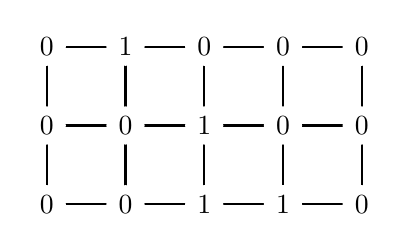
\begin{tikzpicture}
        % row 1
        \cell{0}{0}{1}{1}
        \cell{1}{0}{2}{1}
        \cell{2}{0}{3}{1}
        \cell{3}{0}{4}{1}
        % row 2
        \cell{0}{1}{1}{2}
        \cell{1}{1}{2}{2}
        \cell{2}{1}{3}{2}
        \cell{3}{1}{4}{2}

        \( \lablvertex{0}{0}{$0$} \)
        \( \lablvertex{1}{0}{$0$} \)
        \( \lablvertex{2}{0}{$1$} \)
        \( \lablvertex{3}{0}{$1$} \)
        \( \lablvertex{4}{0}{$0$} \)

        \( \lablvertex{0}{1}{$0$} \)
        \( \lablvertex{1}{1}{$0$} \)
        \( \lablvertex{2}{1}{$1$} \)
        \( \lablvertex{3}{1}{$0$} \)
        \( \lablvertex{4}{1}{$0$} \)

        \( \lablvertex{0}{2}{$0$} \)
        \( \lablvertex{1}{2}{$1$} \)
        \( \lablvertex{2}{2}{$0$} \)
        \( \lablvertex{3}{2}{$0$} \)
        \( \lablvertex{4}{2}{$0$} \)
    \end{tikzpicture}
    \end{center}
\caption{A binary sub-lattice of size $(2,4)$ with index $(011,100)$}
\label{fig:binary sub lattice example}
\end{figure}

Note that for $p>1$, this index does not uniquely define the binary sub-lattice.

As with binary lattices, we can compute $V(\hat{\ell})$ for a binary sub-lattice $\hat{\ell} \in \hat{\mathbb{L}}^{(p,q)}$. We can now define the \textit{state matrix} for $\hat{\mathbb{L}}^{(p,q)}$ to be the $2^{q} \times 2^{q}$ matrix $A^{(p,q)} = (A^{(p,q)}_{i,j})$ where element 

$$A^{(p,q)}_{i,j} = \sum_{\hat{\ell}\text{ with index } (i,j)}V(\hat{\ell}).$$

Here $A_{i,j}$ is the entry in the $i$-th row of the matrix, read top-to-bottom, and in the $j$-th column of the matrix read left-to-right. As the binary sub-lattices $\hat{\mathbb{L}}^{(p,q)}$ with index $(0\dots0,0\dots0)$ are just the binary lattices $\mathbb{L}^{(p,q)}$, we have for a state matrix $A^{(p,q)}$ that 

$$A^{(p,q)}_{0,0} = \sum_{\ell \in \mathbb{L}^{(p,q)}}V(\ell).$$

Theorem \ref{thm: messy mosaics} amounts to an efficient procedure to compute $A^{(p,q)}$.  

\begin{prop}
For the set $\hat{\mathbb{L}}^{(1,q)}$ the associated state matrix $A^{(1,q)}$ can be computed by first defining $A^{(1,2)} = \begin{bmatrix}
7^2 & -1 \\
1 & 1
\end{bmatrix}$. We recursively define $A^{(1,q)} \in \mathbb{Z}^{2^{q} \times 2^{q}}$ given $A^{(1,q-1)}$. Begin by writing
$
A^{(1,k)} = \begin{bmatrix}
A_{[0,0]} & A_{[0,1]} \\
A_{[1,0]} & A_{[1,1]}
\end{bmatrix}
$, where the block matrices $A_{[i,j]}$ are square block matrices of size $2^{k-1} \times 2^{k-1}$. We then have

$$
A^{(1,k+1)} = \begin{bmatrix*}[r]
    7A_{[0,0]} & 7A_{[0,1]} & 7^{-1}A_{[0,0]} & A_{[0,1]} \\
    7A_{[1,0]} & 7A_{[1,1]} & 0A_{[1,0]} & A_{[1,1]} \\
    -7^{-1}A_{[0,0]} & 0A_{[0,1]} & 7^{-1}A_{[0,0]} & A_{[0,1]} \\
    A_{[1,0]} & A_{[1,1]} & -A_{[1,0]} & 7A_{[1,1]} \\
\end{bmatrix*}.
$$

\end{prop}

\begin{proof}
    We use induction on $q$. We can immediately calculate the entries of $A^{(1,2)}$ by listing all size $(1,2)$ binary sub-lattices, then using the definition of $V$. 

    \begin{center}
        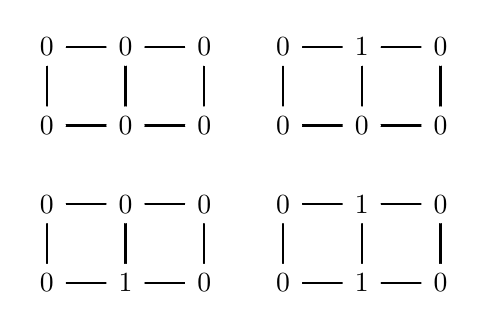
\begin{tikzpicture}
            % row1
            \cell{0}{0}{1}{1}
            \cell{1}{0}{2}{1}

            \cell{3}{0}{4}{1}
            \cell{4}{0}{5}{1}
            % row1
            \cell{0}{2}{1}{3}
            \cell{1}{2}{2}{3}

            \cell{3}{2}{4}{3}
            \cell{4}{2}{5}{3}

            % row 1
            \( \lablvertex{0}{0}{$0$} \)
            \( \lablvertex{1}{0}{$1$} \)
            \( \lablvertex{2}{0}{$0$} \)
            
            \( \lablvertex{0}{1}{$0$} \)
            \( \lablvertex{1}{1}{$0$} \)
            \( \lablvertex{2}{1}{$0$} \)
            
            \( \lablvertex{0}{2}{$0$} \)
            \( \lablvertex{1}{2}{$0$} \)
            \( \lablvertex{2}{2}{$0$} \)
            
            \( \lablvertex{0}{3}{$0$} \)
            \( \lablvertex{1}{3}{$0$} \)
            \( \lablvertex{2}{3}{$0$} \)
            % row 2
            \( \lablvertex{3}{0}{$0$} \)
            \( \lablvertex{4}{0}{$1$} \)
            \( \lablvertex{5}{0}{$0$} \)
            
            \( \lablvertex{3}{1}{$0$} \)
            \( \lablvertex{4}{1}{$1$} \)
            \( \lablvertex{5}{1}{$0$} \)
            
            \( \lablvertex{3}{2}{$0$} \)
            \( \lablvertex{4}{2}{$0$} \)
            \( \lablvertex{5}{2}{$0$} \)
            
            \( \lablvertex{3}{3}{$0$} \)
            \( \lablvertex{4}{3}{$1$} \)
            \( \lablvertex{5}{3}{$0$} \)

            % % arrow
            % \( \lablnode{5.75}{1.5}{$\pmb{\to}$} \)
            % % % matrix
            % \( \lablnode{10}{1.5}{$\begin{bmatrix} v_{(00,00)}v_{(00,00)} & v_{(01,00)}v_{(10,00)} \\ v_{(00,01)}v_{(00,10)} & v_{(01,01)}v_{(10,10)} \end{bmatrix} = \begin{bmatrix} 11^2 & -1 \\ 1 & 1 \end{bmatrix}$} \)
        \end{tikzpicture}
    \end{center}

    Above gives

    $$\begin{bmatrix} v_{(00,00)}v_{(00,00)} & v_{(00,01)}v_{(00,10)} \\ v_{(01,00)}v_{(10,00)} & v_{(01,01)}v_{(10,10)} \end{bmatrix} = \begin{bmatrix} 7^2 & -1 \\ 1 & 1 \end{bmatrix}.$$

    We then assume that the statement for $A^{(1,k)}$ is true up to $k$. Within $A^{(1,k)}$, consider all the size $(1,k)$ binary sub-lattices counted in the entries of the upper left $2^{k-1} \times 2^{k-1}$ block matrix, which we denote $A_{[0,0]}$. By construction, all of these binary sub-lattices have indexes of the form $(0\dots, 0\dots)$, in which both indexes begin with a $0$. Similarly, the upper right $2^{k-1} \times 2^{k-1}$ block matrix $A_{[0,1]}$ counts all binary sub-lattices with indexes like $(0,\dots, 1\dots)$, and so on. 

    To construct binary sub-lattices of size $(1,k+1)$, we then append one of each of the four cells in Figure \ref{fig:four appending cells} to the left of every size $(1,k)$ binary sub-lattices, such that the former left boundary $0$'s are replaced.

    \begin{figure}[h!]
        \begin{center}
            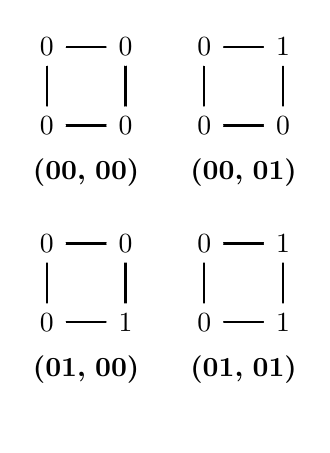
\begin{tikzpicture}
                % row1
                \cell{0}{-0.5}{1}{0.5}
                \cell{2}{-0.5}{3}{0.5}
                % row2
                \cell{0}{2}{1}{3}
                \cell{2}{2}{3}{3}
                % label for row 1
                \( \lablvertex{0}{-0.5}{$0$} \)
                \( \lablvertex{1}{-0.5}{$1$} \)
                \( \lablvertex{2}{-0.5}{$0$} \)
                \( \lablvertex{3}{-0.5}{$1$} \)
                % label for row 2
                \( \lablvertex{0}{0.5}{$0$} \)
                \( \lablvertex{1}{0.5}{$0$} \)
                \( \lablvertex{2}{0.5}{$0$} \)
                \( \lablvertex{3}{0.5}{$1$} \)
                % label for row 3
                \( \lablvertex{0}{2}{$0$} \)
                \( \lablvertex{1}{2}{$0$} \)
                \( \lablvertex{2}{2}{$0$} \)
                \( \lablvertex{3}{2}{$0$} \)
                % label for row 4
                \( \lablvertex{0}{3}{$0$} \)
                \( \lablvertex{1}{3}{$0$} \)
                \( \lablvertex{2}{3}{$0$} \)
                \( \lablvertex{3}{3}{$1$} \)
                % numbers row 1
                \( \lablnode{0.5}{-1.1}{\textbf{(}$\mathbf{01}$\textbf{,} $\mathbf{00}$\textbf{)}} \)
                \( \lablnode{2.5}{-1.1}{\textbf{(}$\mathbf{01}$\textbf{,} $\mathbf{01}$\textbf{)}} \)
                % numbers row 2
                \( \lablnode{0.5}{1.4}{\textbf{(}$\mathbf{00}$\textbf{,} $\mathbf{00}$\textbf{)}} \)
                \( \lablnode{2.5}{1.4}{\textbf{(}$\mathbf{00}$\textbf{,} $\mathbf{01}$\textbf{)}} \)
            \end{tikzpicture}
        \end{center}
        \caption{Appending cells}
        \label{fig:four appending cells}
    \end{figure}

    An example of appending cell $(01,00)$ to the size $(1,3)$ binary sub-lattice $(11,10)$ is shown below.

    \begin{center}
        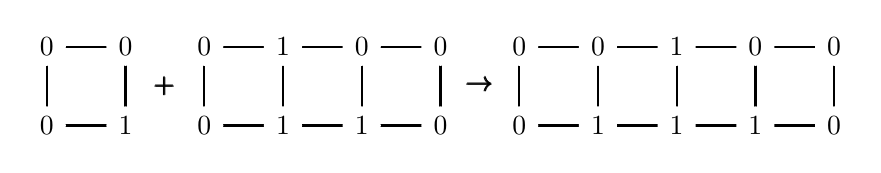
\begin{tikzpicture}
            % row1
            \cell{-1}{0}{0}{1}

            \( \lablnode{0.5}{0.5}{$\pmb{+}$} \)

            \cell{1}{0}{2}{1}
            \cell{2}{0}{3}{1}
            \cell{3}{0}{4}{1}

            \( \lablnode{4.5}{0.5}{$\pmb{\to}$} \)

            \cell{5}{0}{6}{1}
            \cell{6}{0}{7}{1}
            \cell{7}{0}{8}{1}
            \cell{8}{0}{9}{1}

            % row 1
            \( \lablvertex{-1}{0}{$0$} \)
            \( \lablvertex{0}{0}{$1$} \)

            \( \lablvertex{1}{0}{$0$} \)
            \( \lablvertex{2}{0}{$1$} \)
            \( \lablvertex{3}{0}{$1$} \)
            \( \lablvertex{4}{0}{$0$} \)

            \( \lablvertex{5}{0}{$0$} \)
            \( \lablvertex{6}{0}{$1$} \)
            \( \lablvertex{7}{0}{$1$} \)
            \( \lablvertex{8}{0}{$1$} \)
            \( \lablvertex{9}{0}{$0$} \)

            % row 2
            \( \lablvertex{-1}{1}{$0$} \)
            \( \lablvertex{0}{1}{$0$} \)

            \( \lablvertex{1}{1}{$0$} \)
            \( \lablvertex{2}{1}{$1$} \)
            \( \lablvertex{3}{1}{$0$} \)
            \( \lablvertex{4}{1}{$0$} \)

            \( \lablvertex{5}{1}{$0$} \)
            \( \lablvertex{6}{1}{$0$} \)
            \( \lablvertex{7}{1}{$1$} \)
            \( \lablvertex{8}{1}{$0$} \)
            \( \lablvertex{9}{1}{$0$} \)

        \end{tikzpicture}
    \end{center}
    
    This creates the size $(1,4)$ binary sub-lattice $(111,010).$ Notice this operation only changes the identity of the two left-most cells, namely changing the left-most $(01,01)$ cell into cells $(01,00)$ and $(11,01)$. 

    By construction, as every binary sub-lattice counted in the block matrix $A_{[1,1]}$ has an index of the form $(1\dots,1\dots)$, the entries in $A_{[1,1]}$ are all divisible by $v_{01,01}$. Therefore, the size $(1,k+1)$ binary sub-lattices with index of the form $(11\dots,01\dots)$ are counted by $(v_{01,00}v_{11,01}/v_{01,01})A_{[1,1]}$.
    
    Performing the appending operation with each of the four cells from Figure \ref{fig:four appending cells} to each other gives $16$ possible pairs, which we diagram below such that it is consistent with the indexing for $A^{(1,k)}$.

    \begin{center}
        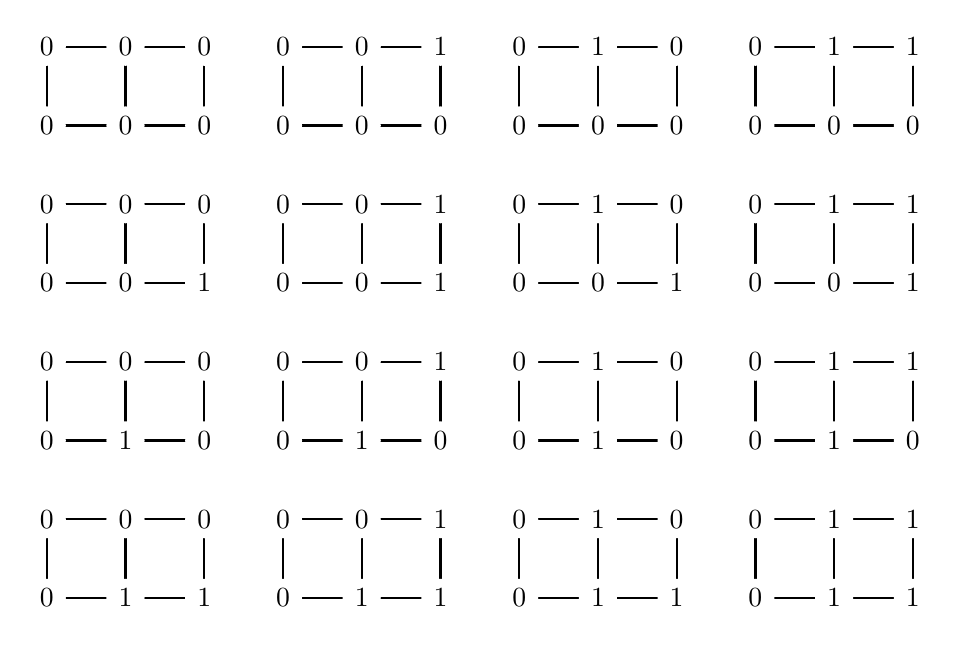
\begin{tikzpicture}
            % row1
            \cell{0}{0}{1}{1}
            \cell{1}{0}{2}{1}
            \( \lablvertex{0}{0}{$0$} \)
            \( \lablvertex{1}{0}{$1$} \)
            \( \lablvertex{2}{0}{$1$} \)
            \( \lablvertex{0}{1}{$0$} \)
            \( \lablvertex{1}{1}{$0$} \)
            \( \lablvertex{2}{1}{$0$} \)
            
            \cell{3}{0}{4}{1}
            \cell{4}{0}{5}{1}
            \( \lablvertex{3}{0}{$0$} \)
            \( \lablvertex{4}{0}{$1$} \)
            \( \lablvertex{5}{0}{$1$} \)
            \( \lablvertex{3}{1}{$0$} \)
            \( \lablvertex{4}{1}{$0$} \)
            \( \lablvertex{5}{1}{$1$} \)

            \cell{6}{0}{7}{1}
            \cell{7}{0}{8}{1}
            \( \lablvertex{6}{0}{$0$} \)
            \( \lablvertex{7}{0}{$1$} \)
            \( \lablvertex{8}{0}{$1$} \)
            \( \lablvertex{6}{1}{$0$} \)
            \( \lablvertex{7}{1}{$1$} \)
            \( \lablvertex{8}{1}{$0$} \)

            \cell{9}{0}{10}{1}
            \cell{10}{0}{11}{1}
            \( \lablvertex{9}{0}{$0$} \)
            \( \lablvertex{10}{0}{$1$} \)
            \( \lablvertex{11}{0}{$1$} \)
            \( \lablvertex{9}{1}{$0$} \)
            \( \lablvertex{10}{1}{$1$} \)
            \( \lablvertex{11}{1}{$1$} \)

            % row2
            \cell{0}{2}{1}{3}
            \cell{1}{2}{2}{3}
            \( \lablvertex{0}{2}{$0$} \)
            \( \lablvertex{1}{2}{$1$} \)
            \( \lablvertex{2}{2}{$0$} \)
            \( \lablvertex{0}{3}{$0$} \)
            \( \lablvertex{1}{3}{$0$} \)
            \( \lablvertex{2}{3}{$0$} \)
            
            \cell{3}{2}{4}{3}
            \cell{4}{2}{5}{3}
            \( \lablvertex{3}{2}{$0$} \)
            \( \lablvertex{4}{2}{$1$} \)
            \( \lablvertex{5}{2}{$0$} \)
            \( \lablvertex{3}{3}{$0$} \)
            \( \lablvertex{4}{3}{$0$} \)
            \( \lablvertex{5}{3}{$1$} \)

            \cell{6}{2}{7}{3}
            \cell{7}{2}{8}{3}
            \( \lablvertex{6}{2}{$0$} \)
            \( \lablvertex{7}{2}{$1$} \)
            \( \lablvertex{8}{2}{$0$} \)
            \( \lablvertex{6}{3}{$0$} \)
            \( \lablvertex{7}{3}{$1$} \)
            \( \lablvertex{8}{3}{$0$} \)

            \cell{9}{2}{10}{3}
            \cell{10}{2}{11}{3}
            \( \lablvertex{9}{2}{$0$} \)
            \( \lablvertex{10}{2}{$1$} \)
            \( \lablvertex{11}{2}{$0$} \)
            \( \lablvertex{9}{3}{$0$} \)
            \( \lablvertex{10}{3}{$1$} \)
            \( \lablvertex{11}{3}{$1$} \)

            % row3
            \cell{0}{4}{1}{5}
            \cell{1}{4}{2}{5}
            \( \lablvertex{0}{4}{$0$} \)
            \( \lablvertex{1}{4}{$0$} \)
            \( \lablvertex{2}{4}{$1$} \)
            \( \lablvertex{0}{5}{$0$} \)
            \( \lablvertex{1}{5}{$0$} \)
            \( \lablvertex{2}{5}{$0$} \)
            
            \cell{3}{4}{4}{5}
            \cell{4}{4}{5}{5}
            \( \lablvertex{3}{4}{$0$} \)
            \( \lablvertex{4}{4}{$0$} \)
            \( \lablvertex{5}{4}{$1$} \)
            \( \lablvertex{3}{5}{$0$} \)
            \( \lablvertex{4}{5}{$0$} \)
            \( \lablvertex{5}{5}{$1$} \)

            \cell{6}{4}{7}{5}
            \cell{7}{4}{8}{5}
            \( \lablvertex{6}{4}{$0$} \)
            \( \lablvertex{7}{4}{$0$} \)
            \( \lablvertex{8}{4}{$1$} \)
            \( \lablvertex{6}{5}{$0$} \)
            \( \lablvertex{7}{5}{$1$} \)
            \( \lablvertex{8}{5}{$0$} \)

            \cell{9}{4}{10}{5}
            \cell{10}{4}{11}{5}
            \( \lablvertex{9}{4}{$0$} \)
            \( \lablvertex{10}{4}{$0$} \)
            \( \lablvertex{11}{4}{$1$} \)
            \( \lablvertex{9}{5}{$0$} \)
            \( \lablvertex{10}{5}{$1$} \)
            \( \lablvertex{11}{5}{$1$} \)

            % row4
            \cell{0}{6}{1}{7}
            \cell{1}{6}{2}{7}
            \( \lablvertex{0}{6}{$0$} \)
            \( \lablvertex{1}{6}{$0$} \)
            \( \lablvertex{2}{6}{$0$} \)
            \( \lablvertex{0}{7}{$0$} \)
            \( \lablvertex{1}{7}{$0$} \)
            \( \lablvertex{2}{7}{$0$} \)
            
            \cell{3}{6}{4}{7}
            \cell{4}{6}{5}{7}
            \( \lablvertex{3}{6}{$0$} \)
            \( \lablvertex{4}{6}{$0$} \)
            \( \lablvertex{5}{6}{$0$} \)
            \( \lablvertex{3}{7}{$0$} \)
            \( \lablvertex{4}{7}{$0$} \)
            \( \lablvertex{5}{7}{$1$} \)

            \cell{6}{6}{7}{7}
            \cell{7}{6}{8}{7}
            \( \lablvertex{6}{6}{$0$} \)
            \( \lablvertex{7}{6}{$0$} \)
            \( \lablvertex{8}{6}{$0$} \)
            \( \lablvertex{6}{7}{$0$} \)
            \( \lablvertex{7}{7}{$1$} \)
            \( \lablvertex{8}{7}{$0$} \)

            \cell{9}{6}{10}{7}
            \cell{10}{6}{11}{7}
            \( \lablvertex{9}{6}{$0$} \)
            \( \lablvertex{10}{6}{$0$} \)
            \( \lablvertex{11}{6}{$0$} \)
            \( \lablvertex{9}{7}{$0$} \)
            \( \lablvertex{10}{7}{$1$} \)
            \( \lablvertex{11}{7}{$1$} \)
        \end{tikzpicture}
    \end{center}

    The associated appending equations for the $v_{i,j}$ values are then

    \begin{align*}
        \frac{v_{(00,00)}v_{(00,00)}}{v_{(00,00)}} = & 7 & \frac{v_{(00,00)}v_{(00,01)}}{v_{(00,01)}} = & 7 & \frac{v_{(00,01)}v_{(00,10)}}{v_{(00,00)}} = & 7^{-1} & \frac{v_{(00,01)}v_{(00,11)}}{v_{(00,01)}} = & 1 \\
        \frac{v_{(00,00)}v_{(01,00)}}{v_{(01,00)}} = & 7 & \frac{v_{(00,00)}v_{(01,01)}}{v_{(01,01)}} = & 7 & \frac{v_{(00,01)}v_{(01,10)}}{v_{(01,00)}} = & 0 & \frac{v_{(00,01)}v_{(01,11)}}{v_{(01,01)}} = & 1 \\
        \frac{v_{(01,00)}v_{(10,00)}}{v_{(00,00)}} = & -7^{-1} & \frac{v_{(01,00)}v_{(10,01)}}{v_{(00,01)}} = & 0 & \frac{v_{(01,01)}v_{(10,10)}}{v_{(00,00)}} = & 7^{-1} & \frac{v_{(01,01)}v_{(10,11)}}{v_{(00,01)}} = & 1 \\
        \frac{v_{(01,00)}v_{(11,00)}}{v_{(01,00)}} = & 1 & \frac{v_{(01,00)}v_{(11,01)}}{v_{(01,01)}} = & 1 & \frac{v_{(01,01)}v_{(11,10)}}{v_{(01,00)}} = & -1 & \frac{v_{(01,01)}v_{(11,11)}}{v_{(01,01)}} = & 7 \\
    \end{align*}
    
    We can then determine
    
    $$
    A^{(1,k+1)} = \begin{bmatrix*}[r]
        7A_{[0,0]} & 7A_{[0,1]} & 7^{-1}A_{[0,0]} & A_{[0,1]} \\
        7A_{[1,0]} & 7A_{[1,1]} & 0A_{[1,0]} & A_{[1,1]} \\
        -7^{-1}A_{[0,0]} & 0A_{[0,1]} & 7^{-1}A_{[0,0]} & A_{[0,1]} \\
        A_{[1,0]} & A_{[1,1]} & -A_{[1,0]} & 7A_{[1,1]} \\
    \end{bmatrix*}.
    $$

\end{proof}

\begin{prop}
    For the set $\mathbb{L}^{(p,q)}$, the state matrix has
    $$A^{(p,q)} = (A^{(1,q)})^p.$$
\end{prop}

\begin{proof}
    We use induction on $p$, and assume $A^{(k,q)} = (A^{(1,q)})^k$. Therefore, 

    $$A^{(k,q)}_{i,j} = \sum_{\hat{\ell}\text{ with index } (i,j)}V(\hat{\ell})$$

    for $\hat{\ell}$ of size $(k,q)$ and index $(i,j)$. Notice that we can build all binary sub-lattices of size $(k+1,q)$ with index $(i,j)$ by the following. Append a size $(1,q)$ binary sub-lattice of index $(i,s)$ and a size $(k,q)$ binary sub-lattice of index $(s,j)$. For example, Figure \ref{fig:appending a row} adjoins a size $(2,3)$ binary sub-lattice with index $(10,01)$ to a size $(1,3)$ binary sub-lattice with index $(01,11)$.

    \begin{figure}[h!]
        \begin{center}
            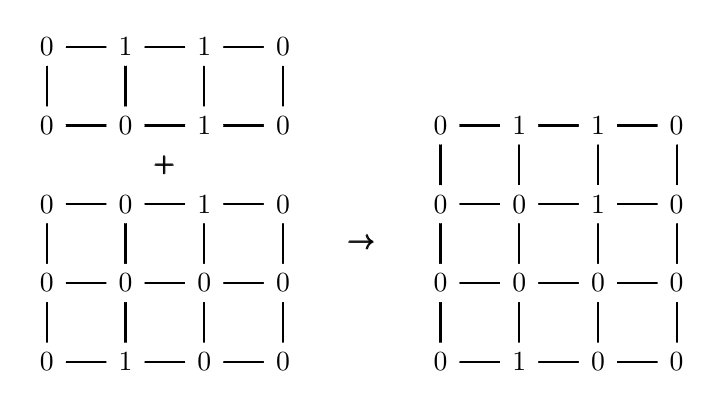
\begin{tikzpicture}
                % row 1
                \cell{0}{0}{1}{1}
                \cell{1}{0}{2}{1}
                \cell{2}{0}{3}{1}
                % row 2
                \cell{0}{1}{1}{2}
                \cell{1}{1}{2}{2}
                \cell{2}{1}{3}{2}
                % row 3
                \cell{0}{3}{1}{4}
                \cell{1}{3}{2}{4}
                \cell{2}{3}{3}{4}

                \( \lablvertex{0}{0}{$0$} \)
                \( \lablvertex{1}{0}{$1$} \)
                \( \lablvertex{2}{0}{$0$} \)
                \( \lablvertex{3}{0}{$0$} \)

                \( \lablvertex{0}{1}{$0$} \)
                \( \lablvertex{1}{1}{$0$} \)
                \( \lablvertex{2}{1}{$0$} \)
                \( \lablvertex{3}{1}{$0$} \)

                \( \lablvertex{0}{2}{$0$} \)
                \( \lablvertex{1}{2}{$0$} \)
                \( \lablvertex{2}{2}{$1$} \)
                \( \lablvertex{3}{2}{$0$} \)

                \( \lablnode{1.5}{2.5}{$\pmb{+}$} \)

                \( \lablvertex{0}{3}{$0$} \)
                \( \lablvertex{1}{3}{$0$} \)
                \( \lablvertex{2}{3}{$1$} \)
                \( \lablvertex{3}{3}{$0$} \)

                \( \lablvertex{0}{4}{$0$} \)
                \( \lablvertex{1}{4}{$1$} \)
                \( \lablvertex{2}{4}{$1$} \)
                \( \lablvertex{3}{4}{$0$} \)

                \( \lablnode{4}{1.5}{$\pmb{\to}$} \)

                % row 1
                \cell{5}{0}{6}{1}
                \cell{6}{0}{7}{1}
                \cell{7}{0}{8}{1}
                % row 2
                \cell{5}{1}{6}{2}
                \cell{6}{1}{7}{2}
                \cell{7}{1}{8}{2}
                % row 3
                \cell{5}{2}{6}{3}
                \cell{6}{2}{7}{3}
                \cell{7}{2}{8}{3}

                \( \lablvertex{5}{0}{$0$} \)
                \( \lablvertex{6}{0}{$1$} \)
                \( \lablvertex{7}{0}{$0$} \)
                \( \lablvertex{8}{0}{$0$} \)

                \( \lablvertex{5}{1}{$0$} \)
                \( \lablvertex{6}{1}{$0$} \)
                \( \lablvertex{7}{1}{$0$} \)
                \( \lablvertex{8}{1}{$0$} \)

                \( \lablvertex{5}{2}{$0$} \)
                \( \lablvertex{6}{2}{$0$} \)
                \( \lablvertex{7}{2}{$1$} \)
                \( \lablvertex{8}{2}{$0$} \)
                
                \( \lablvertex{5}{3}{$0$} \)
                \( \lablvertex{6}{3}{$1$} \)
                \( \lablvertex{7}{3}{$1$} \)
                \( \lablvertex{8}{3}{$0$} \)
            \end{tikzpicture}
        \end{center}
        \caption{Appending a size $(1,3)$ binary sub-lattice to a size $(2,3)$ sub-lattice}
        \label{fig:appending a row}
    \end{figure}

    Doing this append operation for all $s$ amounts to

    $$A_{i,j}^{(k+1,q)} = \sum_{s=0}^{2^{q}-1}A_{i,s}^{(k,q)} A_{s,j}^{(1,q)},$$

    which gives 

    $$A^{(k+1,q)} = A^{(k,q)}A^{(1,q)} = (A^{(1,q)})^{k+1}.$$

\end{proof}

\section{Acknowledgements}

The authors would like to thank Michael Maltenfort for the edits, improvements and ideas for this paper. 

% \newpage

\printbibliography

% \section{Appendix}

% \textbf{TODO}

\end{document}